\section{Introduction}
\subsection{Rappels sur les unités}
En physique atomique et subatomique, on n'utilisera pas les unités classiques que sont le \si{kg}, le \si{m}, etc., mais les unités naturelles, plus appropriées à l'échelle et aux dimensions des structures et phénomènes qui seront étudiés. L'unité de longueur est par exemple le femtomètre (\SI{e-15}{m}), ordre de grandeur du noyau atomique. De plus, on considérera, comme dans le système Heaviside-Lorentz, que  $\hbar=c=\epsilon_0=\mu_0=1$, ce qui transforme quelque peu des expressions familières comme celle de la constante de structure fine, qui devient

\[
    \alpha=\dfrac{e^2}{4\pi\epsilon_0\hbar c}=\dfrac{e^2}{4\pi}\approx\dfrac{1}{137}
\]
Une autre conséquence de cette hypothèse est illustrée dans le tableau ci-dessous: l'unité de masse, qui était précédemment une énergie par vitesse carrée,  devient une énergie, le \si{GeV} et celle de temps, quant à elle, devient l'inverse d'une énergie, le \si{GeV^{-1}}, avec $\SI{1}{GeV^{-1}}=\SI{6.59e-25}{s}$

\begin{table}[H]
    \centering
    \begin{tabu} to 0.7\textwidth {X[2.5,l]X[3.5,l]X[3,l]}
        \hspace*{-3.5mm} (a) & &\\
        \hline\hline
        Quantité & Unité dehaute énergie & Valeur en unité SI \\ \hline
        longueur & \SI{1}{fm} & \SI{e-15}{m} \\
        énergie  & $\SI{1}{GeV} = \SI{e9}{eV}$ & \SI{1.602e-10}{J} \\
        masse, $E/c^2$ & $\SI{1}{GeV}/c^2$ & \SI{1.78e-27}{kg}\\
        $\hbar = h/(2\pi)$ & \SI{6.588e-25}{GeV s} & \SI{1.055e-34}{J s}\\
        $c$ & \SI{2.998e23}{fm s^{-1}} & \SI{2.998e8}{ms^{-1}}\\
        $\hbar c$ & \SI{0.1975}{GeV fm} & \SI{3.162e-26}{J m}\\ \hline\hline \\
    \end{tabu}
    \begin{tabu} to 0.7\textwidth {XX}
        \hspace*{-3.5mm} (b) & \\
        \hline\hline
        \hspace*{-3mm} Unités naturelles; $\hbar = c = 1$ & \\
        masse, $Mc^2/c^2 $ & \SI{1}{GeV} \\
        longueur, $\hbar c/(Mc^2)$ & $\SI{1}{GeV^{-1}} = \SI{0.1975}{fm}$ \\
        temps, $\hbar c/(Mc^3)$ & $\SI{1}{GeV^{-1}} = \SI{6.59e-15}{s}$\\\hline
        \multicolumn{2}{l}{\hspace*{-3mm} Unités Lorentz-Heaviside, $\varepsilon_0 = \mu_0 = \hbar = c = 1$}\\
        constante de structure fine & $\alpha = e^2/(4\pi) \approx 1/137.06$\\\hline\hline
    \end{tabu}
    \caption{Unités naturelles}
    \label{tab:unites_naturelles}
\end{table}

\subsection{Tableau de Mendeleïev}
Le tableau de Mendeleïev (1869) représente tous les éléments chimiques, ordonnés par numéro atomique croissant et organisés en colonnes en fonction de leur configuration électronique, laquelle sous-tend leurs propriétés chimiques.  Le modèle de l'atome comportant des électrons sur des couches permet cette classification des éléments en familles, qui met en évidence la périodicité des propriétés chimiques. Par exemple, la première colonne est celle des Alcalins qui ne comportent qu'un seul électron sur la dernière couche et la dernière colonne est celle des Gaz nobles dont la dernière couche est fermée.

\begin{figure}[ht]
    \centering
    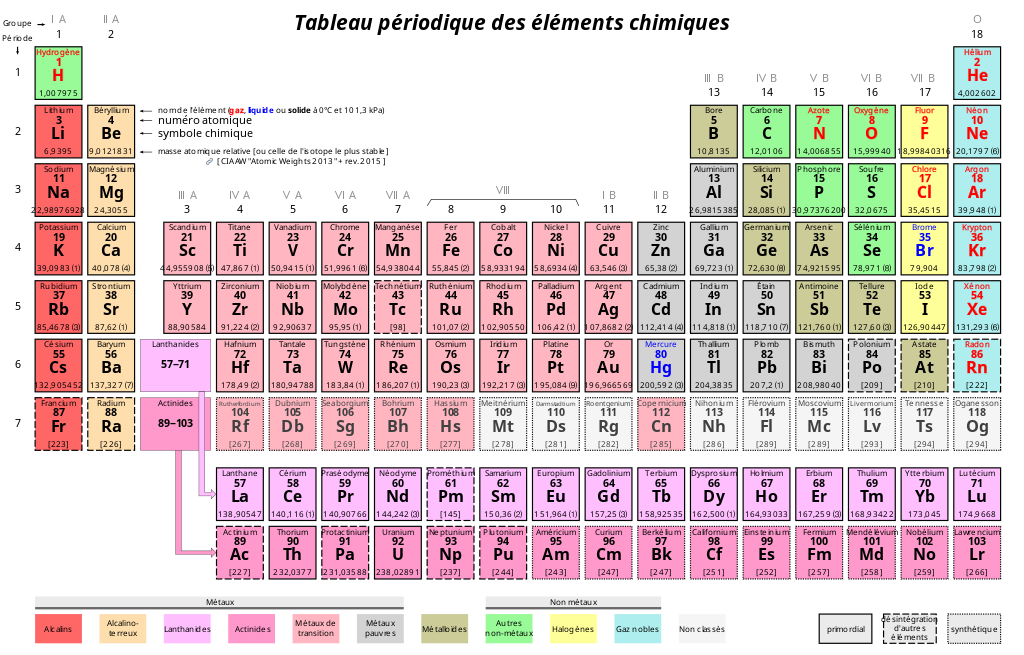
\includegraphics[scale=0.40]{Images1/mend.png}
    \caption{Tableau de Mendeleïev}
\end{figure}

Les atomes se situant dans la même période, c'est-à-dire dans la même ligne du tableau, possèdent le même nombre quantique principal n. Les éléments des mêmes groupes (i.e. même colonne) ont eux des configurations électroniques similaires et donc des propriétés chimiques similaires. On a différents groupes en fonction de la colonne: les métaux alcalins (1), les alcalino-terreux (2) ..., les halogènes (17), les gaz nobles (18). Enfin, les blocs sont des groupes d'éléments dont les électrons de valence occupent des orbitales qui partagent le même nombre quantique $l$ ($l=0,1, \dots, n-1$ correspondant à s, p, d,...).

Les éléments de ce tableau, les atomes, sont des objets très complexes dont la composition (pour le moment admise) est représentée ci-dessous, avec quelques ordres de grandeur. L'électron est un degré de liberté de l'atome, qui possède une charge et un spin, mais pas de position...

\begin{figure}[ht]
    \centering
    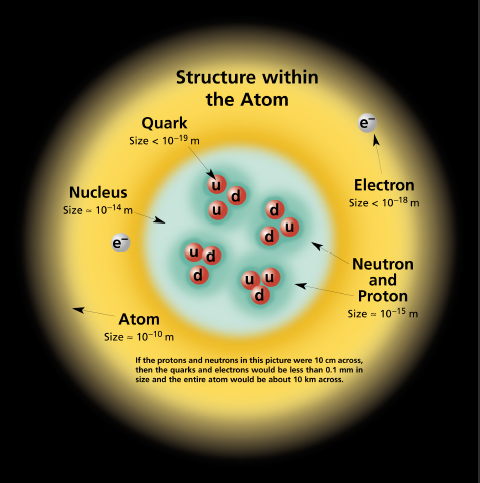
\includegraphics[scale=0.45]{Images1/atome.png}
    \caption{Structure de l'atome}
    \label{fig:struct_atome}
\end{figure}
On admet pour le moment que la matière est constituée de vide et des 4 particules suivantes:

\begin{itemize}
    \item \textbf{les quarks down}, possédant une charge électrique de -1/3
    \item \textbf{les quarks up}, possédant une charge électrique de 2/3
    \item \textbf{les électrons}, de charge -1, responsables des phénomènes électriques et des réactions chimiques
    \item \textbf{les photons}, responsables de l'interaction électromagnétique
\end{itemize}
Protons et neutrons sont composés de quarks: 1 down et 2 up pour le proton, 2 down et 1 up pour le neutron (logique).

\subsection{Modèles de la matière et liens avec la cosmologie et l'astrophysique}
La structure de la matière et l'interaction entre constituants sont intimement liées. En effet, c'est l'interaction entre les rayonnements et la matière qui autorise la description de la structure de celle-ci. Par exemple, les microscopes optiques permettent d'observer des objets de très petite taille, mais leur pouvoir de résolution (i.e leur capacité à séparer des détails très voisins) est limité par le caractère ondulatoire de la lumière, qui engendre de la diffraction. Ainsi, pour voir un objet de taille $d$, il faut un rayonnement dont la longueur d'onde associée $\lambda$ empêche la diffraction, c'est-à-dire telle que
\[ \lambda < d \]
La résolution limite pour de la lumière visible est donc de l'ordre de $\SI{0.5}{\mu m}$.

\subsubsection{Modèles de l'atome}
Différents modèles de plus en plus affinés se sont succédé pour décrire l'atome. Le modèle atomique du <<plum pudding>> fut proposé par J.J. Thomson (Fig \ref{fig:modele_thompson}), qui découvrit l'électron en 1897. Dans ce modèle, l'atome est composé d'électrons plongés dans une <<soupe>> de charges positives pour équilibrer cette charge positive, comme des prunes/raisins selon les versions dans un pudding. Les électrons ne se déplacent pas de façon aléatoire dans l'atome, mais sur des anneaux stabilisés par les interactions entre électrons.

\begin{figure}[ht]
    \centering
    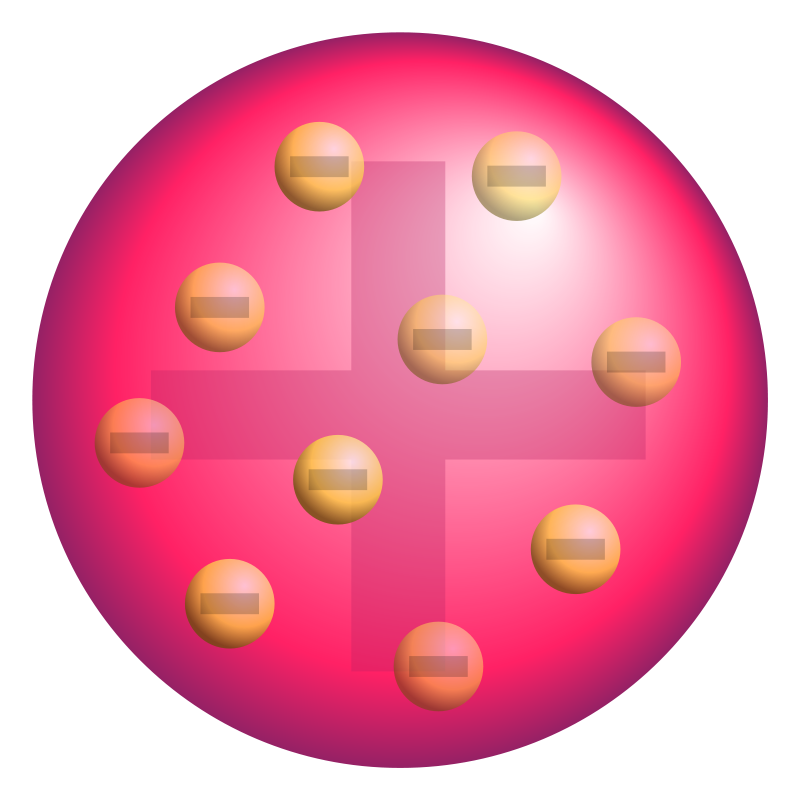
\includegraphics[scale=0.15]{Images1/thomson.png}
    \caption{Modèle de l'atome de Thomson (1897)}
    \label{fig:modele_thompson}
\end{figure}

Ernest Rutherford, considéré comme le père de la physique nucléaire, mit en évidence en 1909 l'existence du noyau atomique, ayant également prouvé au passage l'existence du proton. En 1932, Chadwick découvrit le neutron, remettant ainsi en question le modèle de l'atome. Rutherford imagine donc un atome constitué d'un noyau chargé positivement contenant la majorité de la masse de l'atome et, séparés par du vide, des électrons tournant autour de ce noyau comme des planètes autour d'une étoile (Fig \ref{fig:modele_rutherford}).

\begin{figure}[ht]
    \centering
    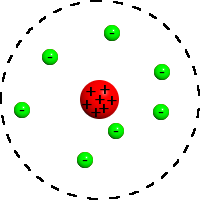
\includegraphics[scale=0.65]{Images1/modelerutherford.png}
    \caption{Modèle de l'atome de Rutherford (1909)}
    \label{fig:modele_rutherford}
\end{figure}

Les accélérateurs actuels (linéaires, circulaires (LHC)) nous permettent d'observer les plus petits constituants de la matière, mais plus la taille de ce que l'on souhaite observer est petite, plus ils doivent être grands, comme illustré ci-dessous. Sur les échelles suivantes sont également représentées les longueurs et énergies, liées par la relation de la longueur d'onde de de Broglie:
\[ \lambda=\dfrac{h}{\sqrt{2mE}} \]
En fait ici c'est un peu complexe, la vraie relation de la longueur d'onde de de Broglie c'est
\[\lambda=\dfrac{h}{p}\]
Ici la relation $p = \sqrt{2mE}$, vient de l'approximation non relativiste $E = \dfrac{p^{2}}{2m}$ (on voit déjà facilement que le cas purement relativiste de la lumière donne une longueur d'onde infinie). L'approximation reste malgré tout correcte assez longtemps (par exemple $v = c/10$ n'est pas du tout relativiste). Selon Lemaître la distinction de régime relativiste doit être faite lorsque l'énergie cinétique commence à être de l'ordre du terme de masse\footnote{Pour rappel, $E = E_\text{cin} + mc^2 = \gamma mc^2$}. Ce terme de masse dépend uniquement de la particule que l'on traite, pour un proton c'est $\SI{938}{MeV}/c^2$ , mais pour un muon c'est $\SI{105.66}{MeV}/c^2$ et un électron c'est 207 fois moins : $\SI{511}{keV}/c^2$. Donc, attention à la formule lorsqu'on dépasse \SI{100}{MeV} pour un proton.

\begin{figure}[ht]
    \centering
    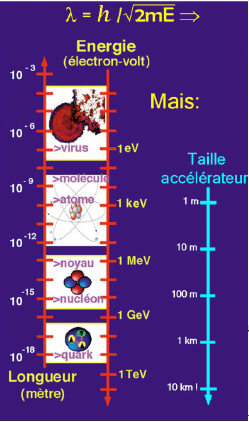
\includegraphics[scale=0.75]{Images1/echelles.png}
    \caption{Relation entre longueur et énergie}
    \label{fig:longeur_energie}
\end{figure}

\subsubsection{Connexion à la cosmologie}
Comprendre les interactions, c'est comprendre l'évolution, du Big Bang à l'apparition de la vie, soit faire de la cosmologie. La théorie du Big Bang de Lemaître et son hypothèse de l'atome primitif ont permis d'établir un lien entre l'infiniment petit (instant juste après le BB) et l'infiniment grand (l'Univers actuel).  Le rayonnement cosmique, la nucléosynthèse primordiale et l'expansion de l'Univers sont des éléments de preuve en faveur de cette théorie.

\begin{figure}[ht]
    \centering
    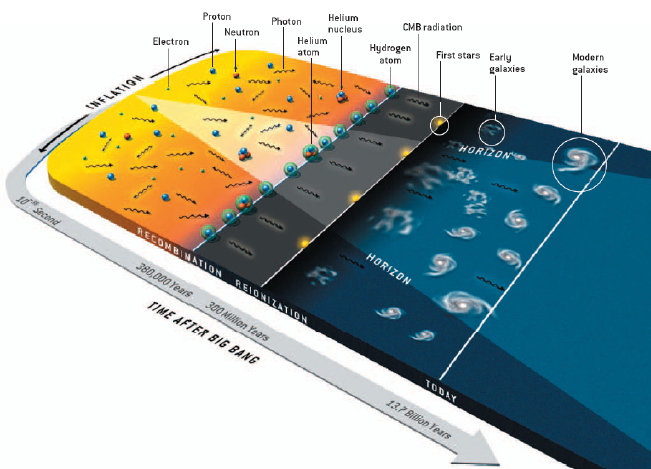
\includegraphics[scale=0.65]{Images1/univers.png}
    \caption{Évolution cosmique}
    \label{fig:evolution_cosmos}
\end{figure}

La ligne du temps de la figure \ref{fig:evolution_cosmos} représente l'évolution de l'Univers depuis le Big Bang. Pendant la première période, on est en présence d'un plasma chaud de gaz ionisé qui se refroidit petit à petit, au fur et à mesure que la nucléosynthèse primordiale se déroule. Elle s'est manifestée à l'échelle de l'Univers tout entier durant les premières dizaines de minutes suivant le Big Bang et est responsable de la formation des noyaux légers, principalement l'hélium 4, mais également le deutérium, une petite partie du lithium et des traces de béryllium. Aucun élément plus lourd n'a été créé durant cette période. Il y a juste déionisation de l'univers, car des atomes se forment.

On remarque ensuite une zone grise entre 380 000 ans et 300 000 millions d'années pendant laquelle l'Univers était <<éteint>>, c'est-à-dire neutre et opaque, il ne se passe rien à part les effets de la gravitation. Remarque: on ne sait pas encore vraiment comment se sont formés les éléments très lourds, car leur synthèse nécessite des conditions très particulières.

Après la période <<d'extinction>>, il y eut formation d'hydrogène et émission de lumière sous forme d'ondes radio, qui ont été détectées par des ingénieurs via des antennes en 1932. On note également le début de la formation des galaxies et des quasars.

Après 1 milliard d'années, l'Univers redevient <<transparent>>, la réionisation est complète,  beaucoup plus d'éléments du tableau périodique sont formés ; les galaxies évoluent. La réionisation a lieu, car les premières étoiles étaient très chaudes, à tel point qu'elles émettent dans l'UV, ce qui peut ioniser les atomes. On assiste à la formation du système solaire vers 9 milliards d'années.\\

On s'intéresse à présent aux premières minutes après le Big Bang au niveau des particules:
\begin{itemize}
    \item $t_0$: instant du Big Bang
    \item $t_0 + \SI{e-34}{s}$: compliqué, relève de la théorie des cordes et de la gravité quantique à boucles.
    \item $t_0 + \SI{e-12}{s}$: énergie de \SI{1}{TeV}, soupe de particules élémentaires (bosons W, quarks en tout genre, muons, positrons...). Il y a une légère asymétrie entre matière et antimatière, qui n'est toujours pas comprise à l'heure actuelle. Un peu après, il ne reste plus assez d'énergie pour créer une paire quark-antiquark, il reste donc quelques quarks tout seuls.
\end{itemize}

\begin{figure}[ht]
    \centering
    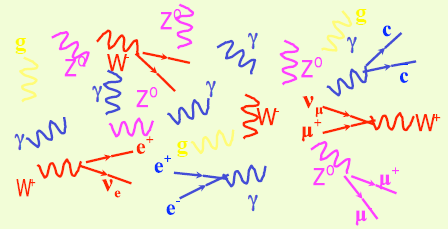
\includegraphics[width=0.45\textwidth]{Images1/soupe.png}
    \caption{Soupe primordiale}
    \label{fig:soupe_promordiale}
\end{figure}

\begin{rem}
    Comment peut-on affirmer avec certitude qu'il n'existe pas d'anti-monde rempli d'antimatière (une anti-galaxie avec un anti-soleil, etc.) ? Car il provoquerait des effets gravitationnels et électromagnétiques tellement cataclysmiques qu'on ne pourrait pas les rater.
\end{rem}

\begin{itemize}
    \item $t_0 + \SI{e-2}{s}$: énergie de \SI{1}{GeV}, mariage des quarks et formation des nucléons sous l'effet de l'interaction forte (neutron = 2 down + 1 up, proton = 2 up + 1 down)
    \item $t_0+ \SI{100}{s}$: \SI{100}{eV} ($10^9$ degrés), existence d'états liés entre neutrons et protons sous l'effet de l'interaction faible, comme le deutérium et l'hélium (noyaux légers).
\end{itemize}

\begin{figure}[ht]
    \centering
    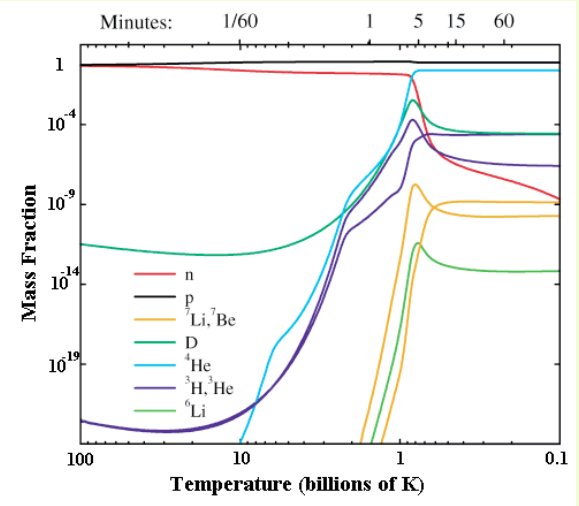
\includegraphics[scale=0.50]{Images1/tempmass.png}
    \caption{Évolution des proportions d'éléments en fonction du temps}
\end{figure}

\begin{itemize}
    \item $t_0+30$ min: le contenu de l'Univers est dominé par les protons et l'hélium (il y a aussi des électrons et photons). On est en présence d'un plasma électriquement neutre (Fig. \ref{fig:BB_30mn}).
    \item $t_0 + 300.000$ ans: les photons sont libres, on les observe
    \item $t_0 + 700.000$ ans: 3000 degrés, formation des atomes les plus simples sous l'effet de l'interaction électromagnétique
\end{itemize}

\begin{figure}[ht]
    \centering
    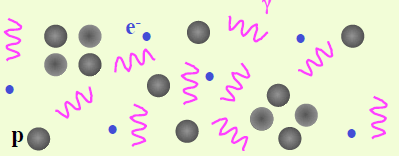
\includegraphics[scale=0.50]{Images1/30min.png}
    \caption{Univers 30 minutes après le Big Bang}
    \label{fig:BB_30mn}
\end{figure}

% \textcolor{blue}{[Revoir cette section]}
\subsubsection{Connexion à l'astrophysique}
En ce qui concerne la connexion à l'astrophysique, la structure microscopique de la matière permet une compréhension très riche des astres et du cosmos.

Par exemple le Nuage d'Orion est relativement proche de la Terre dans la Voie lactée. L'observation de son spectre permet de conclure sur sa composition en certains atomes et molécules. De telles conclusions ne seraient pas possibles sans la connaissance du monde microscopique pour décrypter ces observations.


\section{Structure de la matière}
Cette section porte sur la découverte de particules et de rayonnements, ainsi que sur leurs pertes d'énergie. Il est donc bon de commencer par restituer différents évènements sur une ligne du temps (Fig. \ref{fig:decouvertes}):

\begin{figure}[ht]
    \centering
    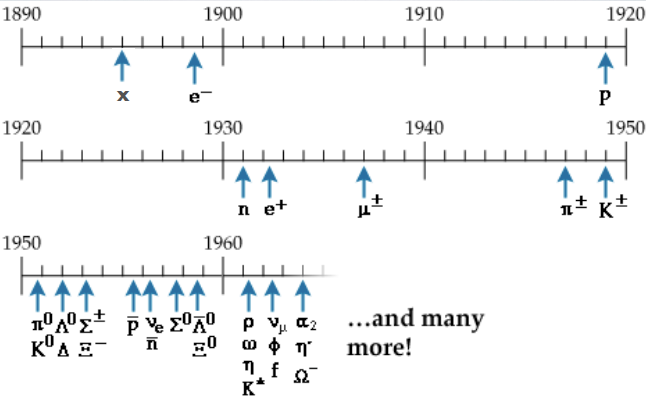
\includegraphics[scale=0.50]{Images1/ldt.png}
    \caption{Découverte de différentes particules et rayonnements}
    \label{fig:decouvertes}
\end{figure}

\begin{itemize}
    \item 1895: Découverte des rayons X (Roentgen)
    \item 1896: Découverte de la radioactivité (Becquerel)
    \item 1897: Découverte de l'électron (J.J. Thomson)
    \item 1909: Preuve que les particules $\alpha$ sont de noyaux d'hélium (Rutherford)
    \item 1911: Découverte du noyau (Rutherford)
    \item 1912: Découverte des rayonnements cosmiques (Hess)
    \item 1928: Théorie de l'$\alpha$-radioactivité (Gamow, Gurney, Condon)
    \item 1930: Hypothèse du neutrino (Pauli)
    \item 1932: Découverte du neutron (Chadwick)
    \item 1934: Théorie de la $\beta$-radioactivité (Fermi)
    \item ...
\end{itemize}


\subsection{Des rayons X à la découverte de l'électron}
\subsubsection{Fluorescence et phosphorescence}
Une molécule fluorescente possède la propriété d'absorber de l'énergie lumineuse (lumière d'excitation) et de la restituer rapidement sous forme de lumière fluorescente (lumière d'émission). Une fois l'énergie du photon absorbée, la molécule se trouve alors généralement dans un état électroniquement excité, souvent un état singulet, noté S1. (L'état fondamental qui est aussi singulet est noté S0.) Le retour à l'état fondamental peut alors se faire de différentes manières : soit par fluorescence, soit par phosphorescence (Fig. \ref{fig:fluorescence_phosphorescence}).

La fluorescence est caractérisée par l'émission d'un photon de manière très rapide. Cette rapidité s'explique par le fait que l'émission respecte une des règles de sélection de l'émission de photons de la mécanique quantique qui est $\Delta S=0$, ce qui signifie que la molécule reste dans un état singulet.

La phosphorescence quant à elle est caractérisée par une transition d'un état S=0 vers un état S=1 (état triplet noté T1), qui n'est pas permise par le modèle quantique, mais qui est rendue possible par le couplage spin-orbite. Cependant, la transition est plus lente à s'effectuer. Suit alors une émission de photon pour retourner à l'état fondamental.

\begin{figure}[ht]
    \centering
    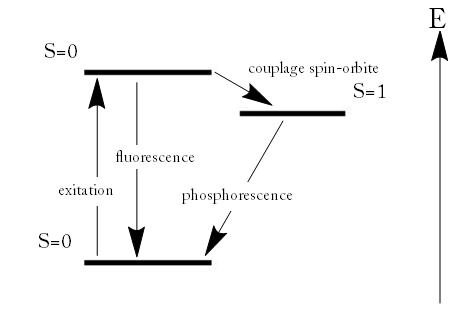
\includegraphics[scale=0.65]{Images1/fluophospho.jpg}
    \caption{Fluorescence VS phosphorescence}
    \label{fig:fluorescence_phosphorescence}
\end{figure}

\subsubsection{Découverte des rayons X (Röntgen, 1895, PN en 1901)}
Les rayons X sont une forme de rayonnement électromagnétique à haute fréquence constitué de photons. L'énergie de ces photons va d'une centaine d'$eV$ à environ un $\si{MeV}$. Anecdote: Röntgen les a appelés rayons <<X>> en référence à l'inconnue mathématique.

Ils sont de même nature que les rayons gamma, mais produits différemment : les rayons X sont produits par des transitions électroniques alors que les rayons gamma proviennent de la désintégration radioactive des noyaux des atomes.

Comment Röntgen les a-t-il découverts? Comme beaucoup de physiciens à l'époque, il se passionnait pour les <<rayons cathodiques>>, étudiés auparavant par William Crookes via les célèbres <<tubes de Crookes>>.

\begin{figure}[ht]
    \centering
    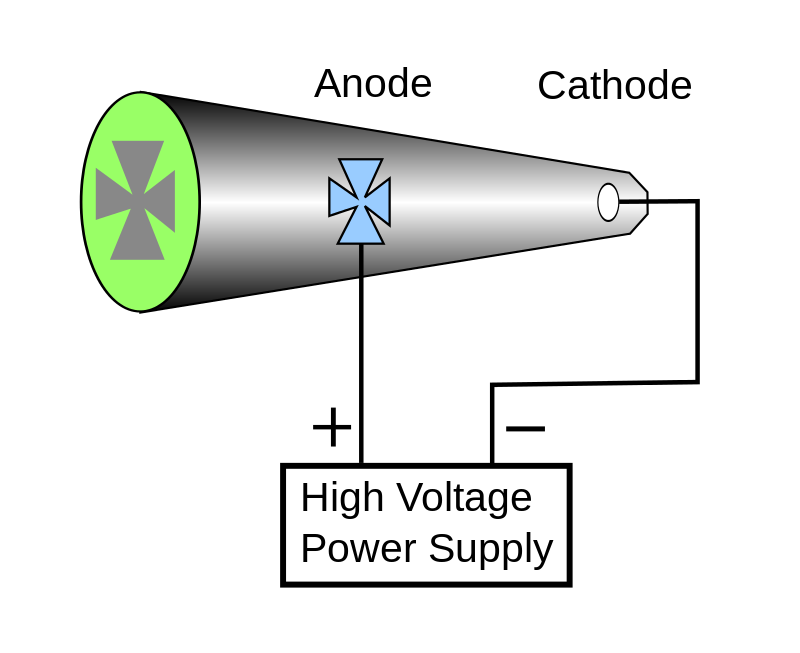
\includegraphics[scale=0.20]{Images1/tubecrookes.png}
    \caption{Schéma d'un tube de Crookes}
\end{figure}

Le tube de Crookes est un tube de verre froid sous vide partiel possédant 2 électrodes de métal, une à chaque extrémité. Quand on applique une forte tension électrique entre les électrodes, le champ électrique induit l'accélération des ions chargés présents dans le gaz résiduel. Ils entrent en collision avec les autres molécules du gaz, leur arrachant au passage des électrons, ce qui crée des cations. Ces derniers sont attirés par la cathode (électrode négative). À l'instant où ils la percutent, ils éjectent un grand nombre d'électrons de la surface métallique, qui sont eux attirés par l'électrode positive, l'anode. Ces électrons sont ce qu'on a appelé plus haut les <<rayons cathodiques>>. Il y a donc un faisceau d'électrons qui traverse le tube depuis la cathode vers l'anode.

Quand on applique une différence de potentiel supérieure ou égale à \SI{5 000}{V} à un tube de Crookes, les électrons sont accélérés à une vitesse telle qu'un rayonnement est émis de l'anode vers le récepteur. Le spectre de ce rayonnement est continu et comporte des pics. Il montre 2 caractéristiques témoignant de 2 phénomènes différents:

\begin{itemize}
    \item \textbf{Le rayonnement continu de freinage (ou Bremsstrahlung)} : les électrons accélérés émettent des rayons X au moment où ils passent à proximité de la charge électrique portée par le noyau atomique des molécules composant la cible et que leur trajectoire est brutalement infléchie. (car ils sont décéléré par le champ électrique des noyaux)
    \item \textbf{la fluorescence X} : quand les électrons rencontrent les <<électrons profonds>> d'un atome de la paroi du tube, ils les placent dans des niveaux d'énergie plus élevés, car ils leur arrachent des électrons sur la couche externe. Les électrons de l'atome doivent alors redescendre d'un niveau d'énergie pour se stabiliser, émettant au passage des rayons X.
\end{itemize}

En 1895, Röntgen manipulait un tube de Crookes recouvert d'un carton noir quand il s'aperçut qu'un des écrans scintillants situé à proximité du tube scintillait un peu. Il en déduit que les rayons issus du tube étaient capables de traverser le carton et faire fluorescer l'écran, même dans l'obscurité. Il observa aussi que les rayons traversaient ses livres et papiers, mais qu'il était plus ou moins pénétrant en fonction de la densité de l'objet à traverser. \\

Aujourd'hui, on produit les rayons X dans des tubes spéciaux (tubes à rayons X figure \ref{fig:tube_rayon_x}) qui sont en quelque sorte une évolution des tubes de Crookes. Contrairement à ces derniers, ils sont chauffés. Une haute tension est établie entre deux électrodes. Il se produit alors un courant d'électrons de la cathode vers l'anode comme expliqué plus haut. Les électrons sont freinés par les atomes de la cible, ce qui provoque un rayonnement continu de freinage ou Bremsstrahlung, dont une partie du spectre est dans le domaine des rayons X. Ces électrons excitent les atomes de la cible, et ceux-ci réémettent un rayonnement X caractéristique par le phénomène de fluorescence X. Le spectre sortant du tube est donc la superposition du rayonnement de freinage et de la fluorescence X de la cible (voir figure \ref{fig:spectre_rayon_x}). Le système représenté en bleu sur le schéma ci-dessous est un dispositif de circulation d'eau pour refroidie le tube, car la dissipation de chaleur est énorme, bien qu'aujourd'hui cet effet soit mieux contrôlé, notamment en faisant tourner l'anode pour qu'elle ne soit pas toujours percutée au même endroit. La bobine est souvent en tungstène.

\begin{figure}[ht]
    \centering
    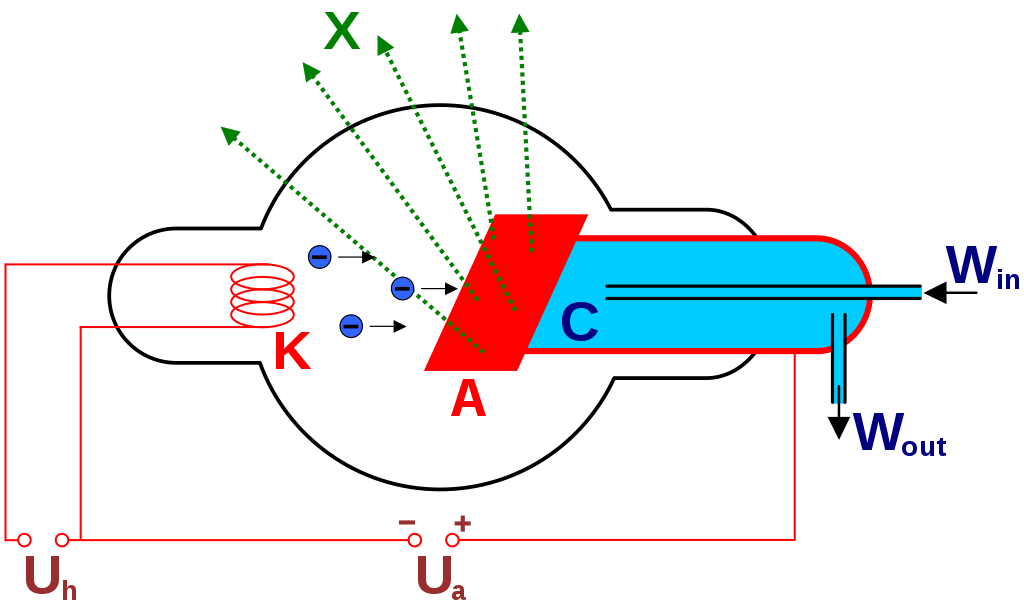
\includegraphics[width=0.5\textwidth]{Images1/rayonsxtube.png}
    \caption{Production de rayons X dans un tube à anode fixe}
    \label{fig:tube_rayon_x}
\end{figure}

\begin{figure}[ht]
    \centering
    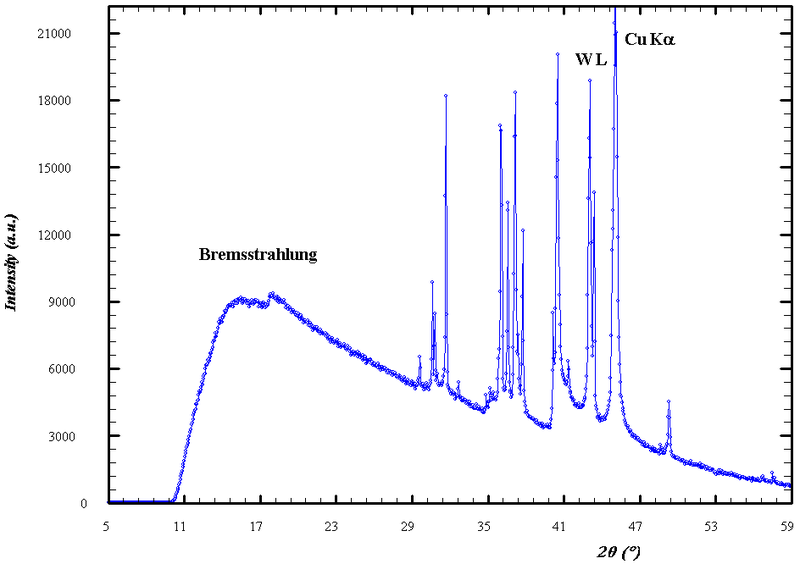
\includegraphics[scale=0.30]{Images1/rayonnement.PNG}
    \caption{Composition du spectre sortant du tube à rayons X}
    \label{fig:spectre_rayon_x}
\end{figure}

\subsubsection{Découverte de la radioactivité naturelle (Becquerel, 1896, PN en 1903)}
En 1896, Henri Becquerel cherche à déterminer si le phénomène de fluorescence des sels d'uranium est de même nature que les rayons X. Il dépose des sels phosphorescents d'uranium sur des plaques photographiques, elles-mêmes enveloppées dans du papier noir et les expose au soleil. Les photographies révèlent l'image des cristaux de sel d'uranium. Becquerel pense donc que l'énergie du soleil est absorbée par l'uranium avant d'être réémise sous forme de rayons X.

Cependant, un jour de mauvais temps, Becquerel doit renoncer à reproduire son expérience et il range donc ses plaques photographiques imprégnées de sels d'uranium dans un placard. Surprise, quelques jours plus tard, les plaques sont quand même impressionnées et Becquerel distingue même l'image négative d'une croix de cuivre qui se trouvait entre l'uranium et l'une de ses plaques photographiques. Il ne peut donc que conclure qu'une substance inerte se montre capable d'émettre des rayons, en l'absence de lumière, qui traversent le papier, mais sont tout de même arrêtés par le métal. \\

On a une loi de comportement pour décrire la désintégration radioactive: dans une boîte avec $N$ particules, le taux de désintégration ne change pas. C'est assez contre-intuitif par rapport à la nature, car si on fait une analogie avec notre classe, dans 50 ans, quelques-uns auront disparu à cause du vieillissement, mais ce nombre de disparus sera encore bien plus important dans 100 ans (rip). \textbf{Cette notion de vieillissement n'existe pas chez les particules}, elles se désintègrent au même taux à tout moment:
\[    \Delta N(t)=-\lambda N(t) \Delta t    \]
où
\begin{itemize}
    \item $N(t)$ est le nombre de noyaux radioactifs de l'espèce initiale existant à l'instant $t$. On suppose qu'il ne varie que très peu dans l'intervalle de temps $[t,t+\Delta t]$
    \item $\Delta N(t)$ est le nombre de noyaux qui se transforment pendant l'intervalle de temps $[t,t+\Delta t]$
    \item $\lambda$ est une constante de proportionnalité ayant les dimensions de l'inverse d'un temps, appelée constante radioactive (remarquons qu'elle ne dépend pas du temps: les atomes ne vieillissent pas)
\end{itemize}
On a donc
\[
    \fdif{N(t)}{t}=-\lambda N(t)
\]
ou encore
\[
    N(t)=N(0)e^{-\lambda t}
\]
N.B: une fois qu'ils ont découvert la radioactivité et ses <<pouvoirs curatifs miraculeux>>, les gens se sont un peu emballés...

\begin{figure}[H]
    \centering
    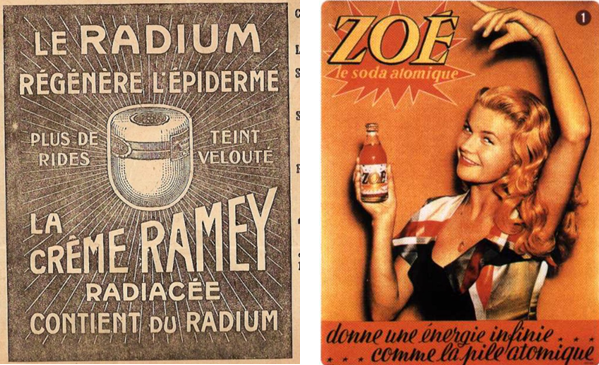
\includegraphics[scale=0.60]{Images1/produits.png}
    \caption{Crème et soda radioactifs}
\end{figure}

\subsubsection{Découverte de l'électron (Thomson, 1897, PN en 1906)}
Les tubes de Crookes furent utilisés dans de très nombreuses expériences afin de déterminer la nature des rayons cathodiques. Deux théories coexistaient : Crookes croyait qu'il s'agissait de <<corpuscules>> ou <<matière radiante>> c'est-à-dire d'atomes chargés électriquement. D'autres chercheurs pensaient qu'il s'agissait de vibrations de l'éther, une nouvelle forme de rayonnement électromagnétique. Le débat continua jusqu'à ce que J. J. Thomson mesure leur masse, prouvant qu'ils avaient affaire à des particules chargées négativement inconnues auparavant, qu'il appela <<corpuscules>>, mais qui furent plus tard appelées électrons. En 1869, on construisit une anode avec une forme de croix de Malte dans le tube. Lorsque le tube était allumé, il projetait une ombre en forme de croix sur la matière fluorescente dans la partie arrière du tube (figure \ref{fig:croix_de_malte}), montrant que les rayons se déplaçaient en ligne droite.

\begin{figure}[ht]
    \centering
    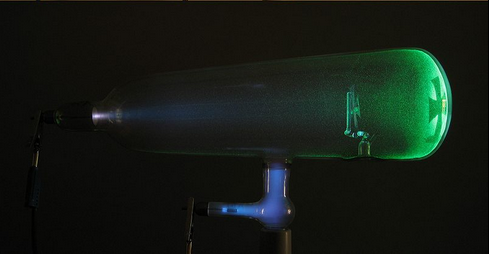
\includegraphics[scale=0.60]{Images1/croixmalte.PNG}
    \caption{Expérience de la croix de Malte}
    \label{fig:croix_de_malte}
\end{figure}

La preuve expérimentale de l'existence des électrons est le résultat de 3 expériences menées par Thomson:

\begin{itemize}
    \item Première expérience: Il cherche à savoir si on peut séparer la charge négative des rayons cathodiques par le biais du magnétisme. La conclusion est que ce n'est pas le cas. (d'où <<interprétation corpusculaire des rayons cathodiques>>)
    \item Deuxième expérience: Il prouve que les rayons cathodiques peuvent être déviés par un champ électrique. Il construit un tube cathodique muni d'une couche de peinture phosphorescente au bout pour détecter des rayons incidents. Thomson démontre une déviation dans un sens, qui indique que la charge des rayons cathodiques est négative. (Fig. \ref{fig:thompson_exp_2})

    \begin{figure}[ht]
        \centering
        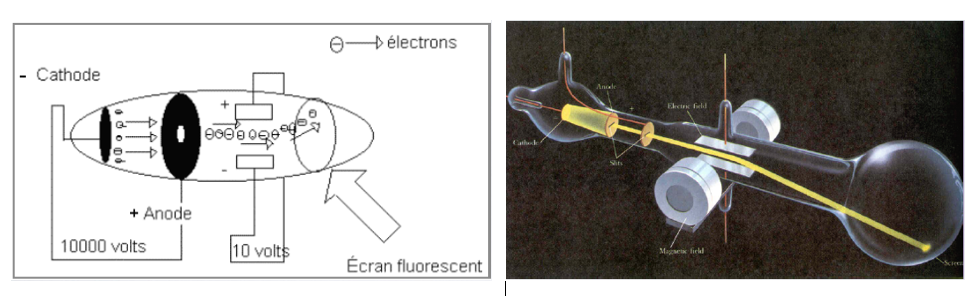
\includegraphics[scale=0.60]{Images1/2eexpthomson.PNG}
        \caption{Deuxième expérience de Thomson - Dispositif expérimental}
        \label{fig:thompson_exp_2}
    \end{figure}

    \item Troisième expérience: Détermination du rapport charge/masse $(e/m)$. Pour déterminer ce rapport, Thomson mesure la déviation et l'énergie cinétique des rayons cathodiques sous l'influence du champ magnétique. Son calcul lui donne un résultat pour $e/m$ mille fois plus élevé que le rapport analogue pour un ion hydrogène, ce qui suggère que les rayons cathodiques contiennent des particules soit très légères soit très hautement chargées. Thomson arrive à la conclusion que les rayons cathodiques sont composés de <<corpuscules>> qui proviennent de l'intérieur des atomes des électrodes, ce qui implique que les atomes sont divisibles. Le <<corpuscule>> découvert par Thomson est l'électron.
    S'en suit la proposition de modèle du <<plum pudding>> pour l'atome.
\end{itemize}

\subsubsection{Détermination de la charge de l'électron}
Elle se fit via l'expérience de la goutte d'huile de Millikan, qui consiste à pulvériser de minuscules gouttes d'huiles électrisées entre les 2 électrodes horizontales d'un condensateur plan chargé. Les gouttes sont soumises à plusieurs forces qui s'équilibrent rapidement, elles se déplacent donc à une vitesse constante qu'on peut mesurer.

\begin{figure}[ht]
    \centering
    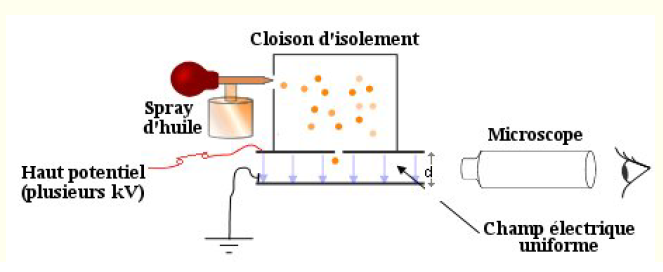
\includegraphics[scale=0.60]{Images1/millikan.PNG}
    \caption{Expérience de la goutte d'huile de Millikan}
\end{figure}

Le principe est de sélectionner une goutte, et  d'analyser son mouvement sous l'action des forces agissant sur elle  à différentes valeurs d'ionisation.

Millikan, mesura la vitesse d'une gouttelette d'huile qu'il ionisait en l'irradiant grâce à des rayons X. Cette mesure de la vitesse fut déterminée par le rapport entre la distance parcourue par la gouttelette d'huile et le temps mis pour effectuer ce déplacement. Ses observations lui firent se rendre compte que toutes les valeurs d'ionisation étaient multiples entiers de $e=\SI{1.592e-19}{C}$, que l'on définit comme la charge élémentaire.

\paragraph{Détails:} Si on modélise simplement le problème, la goutte d'huile subit les 4 forces suivantes:
\begin{itemize}
    \item Son poids $\Vec{P}=\dfrac{4}{3}\pi r^3 \rho_h\Vec{g}$
    \item La force électrostatique $\Vec{F_E}=q\Vec{E}$
    \item La poussée d'Archimède $\Vec{F_A}=-\dfrac{4}{3}\pi r^3 \rho_a \Vec{g}$
    \item La force de trainée (résistance de l'air) $\Vec{F_R}=-6\pi\eta r\Vec{v}$ où $\eta$ est le coefficient de viscosité de l'air et $v$ la vitesse de la gouttelette.
\end{itemize}
On peut mesurer la charge $q$ de la goutte de différentes façons. Considérons la méthode du champ constant, dans laquelle on garde l'amplitude du champ constante et on alterne la polarité du condensateur, de sorte que la force électrique soit dirigée tantôt vers le haut, tantôt vers le bas. \\[0,2cm]
Dans le cas de la force électrique vers le haut (vitesse $v_1$), on a
\begin{equation}
    qE+F_A = mg+6\pi\eta rv_1
    \label{eq:force_elec_haut}
\end{equation}
    Pour la force électrique vers le bas (vitesse $v_2$),
\begin{equation}
    qE+mg = 6\pi\eta rv_2 + F_A
    \label{eq:force_elec_bas}
\end{equation}
Si on soustrait (\ref{eq:force_elec_haut}) et (\ref{eq:force_elec_bas})
\[
    2(mg-F_A)=6\pi\eta r(v_2-v_1)
\]
vu que

\[
mg-F_A=\dfrac{4\pi}{3}r^3g(\rho_h-\rho_a)\quad\text{et}\quad
r=\dfrac{3}{2}\sqrt{\dfrac{\eta(v_2-v_1)}{g(\rho_h-\rho_a)}}
\]
Si on additionne (\ref{eq:force_elec_haut}) et (\ref{eq:force_elec_bas}), on obtient
\[
    2qE=6\pi\eta r(v_2+v_1)
\]
donc
\[
    q=\dfrac{9\pi}{2E}\sqrt{\dfrac{\eta^3(v_2-v_1)}{g(\rho_h-\rho_a)}}(v_2+v_1)
\]
Si on effectue 2 mesures de vitesse pour une goutte donnée, on peut donc déterminer $q$.

\subsection{Perte d'énergie dans la matière}

L'intérêt de l'étude de la perte d'énergie lors d'une interaction particule-matière réside dans le fait que c'est l'outil principal de détection de particule. Commençons par étudier la perte d'énergie des particules lourdes, c'est-à-dire des particules possédant une masse bien supérieure à celle de l'électron. Si elles ont une énergie basse, la perte d'énergie est dominée par leur interaction électromagnétique avec les électrons atomiques: il y a excitation et/ou ionisation de l'atome par transfert d'une partie de l'énergie cinétique de la particule incidente. Si au contraire elles ont une haute énergie, ce sont les interactions nucléaires qui sont importantes.

\subsubsection{Perte d'énergie par ionisation}
La section efficace (cfr section \ref{sec:section_efficace}) étant très petite (de l'ordre de \SI{e-17}{cm^2}), la probabilité de collision est très faible, mais la grande densité d'atomes ($N_A=\SI{6.02e23}{\mole^-1}$) dans un matériau rend la perte d'énergie totale très importante, même pour une faible épaisseur. Par exemple, un proton de 10 \si{MeV} perd toute son énergie dans \SI{0.25}{mm} de cuivre !

L'énergie est perdue par la particule dans des <<collisions inélastiques>> avec les électrons des atomes du matériau. On a un très grand nombre de collisions, par conséquent l'énergie perdue par collision est petite. On dit qu'on a affaire à une diminution \textbf{continue} d'énergie. À la fin du parcours, les électrons sont capturés par la particule jusqu'à ce que l'énergie de cette dernière soit de l'ordre de l'énergie thermique des atomes du milieu.

\begin{rem}
    Le phénomène est décrit à l'aide du terme collision, mais il n'y a pas nécessairement contact entre l'électron incident (ou la particule chargée) et l'électron de l'atome cible. Néanmoins, le phénomène résultant de cette interaction électrostatique de durée très brève peut s'apparenter à une collision.
\end{rem}

Calculons la perte d'énergie se faisant lors du passage à travers une couche $\dif x$ de matière, comme représenté sur la figure \ref{fig:interraction_particule_matiere}.
\begin{figure}[ht]
    \centering
    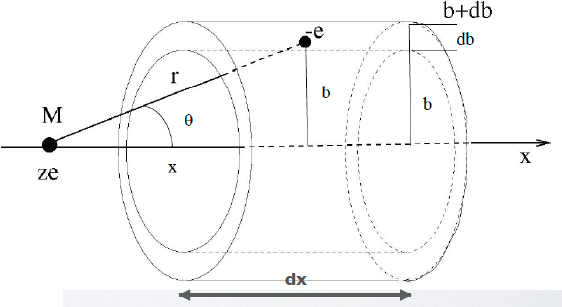
\includegraphics[scale=0.60]{Images1/pertenrj.PNG}
    \caption{Interaction entre particule (ze) et électron de matière}
    \label{fig:interraction_particule_matiere}
\end{figure}
L'impulsion verticale fournie par la particule incidente à un électron atomique à travers la force de Coulomb est
\[
    \Delta P_t=\int_{-\infty}^\infty F_y \dt=\int_{-\infty}^\infty \dfrac{ze^2}{4\pi \epsilon_0 r^2} \sin{\theta}\dfrac{\dif x}{v}
\]
où
\[\begin{cases}
    \dfrac{1}{r^2} &= \dfrac{\sin^2\theta}{b^2} \\[2mm]
    x &= \dfrac{b}{\tan{\theta}} \\[2mm]
    \dif x &= -\dfrac{b}{(\sin{\theta})^2}\dif\theta
\end{cases}\]
Ainsi
\[
    \Delta P_t=\int_{0}^\pi \dfrac{ze^2}{4\pi \epsilon_0}\dfrac{\sin{\theta}}{vb}\dif\theta = \dfrac{ze^2}{2\pi \epsilon_0 vb}
\]
Dans une approche non relativiste, l'énergie transmise à l'électron est
\[
    \dif E_E=\dfrac{p^2}{2m_e}=\dfrac{z^2e^4}{8\pi^2{\epsilon_0}^2v^2b^2m_e}
\]
En admettant une distribution uniforme des électrons, le nombre de <<collisions>> que la particule subit avec des électrons situés à un paramètre d'impact compris entre $b$ et $b+\dif b$ dans une épaisseur $\dif x$ est\footnote{$A$ est la masse molaire, $\dfrac{\rho N_A}{A}$ est donc le nombre d'atomes du milieu par unité de volume.}
\[
    \dif N_e=\dfrac{\rho N_A}{A}Z(2\pi b \dif b \dif x)
\]
qui engendre un transfert d'énergie
\[
    \dif T_e=\dif N_e\dif E_e=\dfrac{z^2e^4}{4\pi \epsilon_0^2v^2bm_e}\Big(\dfrac{\rho N_A}{A}\Big)Z \dif b \dif x
\]
Par unité de distance, on a donc la perte d'énergie
\[
    -\fdif{E}{x}=\int_{b_\text{min}}^{b_\text{max}} \fdif{T_e(b)}{x}=\Big(\dfrac{\rho N_A}{A}\Big)Z\dfrac{z^2e^4}{4\pi \epsilon_0^2m_ev^2}\ln{\Big(\dfrac{b_\text{max}}{b_\text{min}}\Big)}
\]
Cependant, on a un problème puisque cette intégrale diverge. On doit donc en limiter les bornes en utilisant des arguments qualitatifs à savoir les estimations de $b_\text{min}$ et $b_\text{max}$:

\begin{itemize}[label=$\rightarrow$]
    \item \underline{\textbf{b grand $\Leftrightarrow\Delta E(b)$ petit}}\\[0,2cm]
    Les électrons sont liés aux noyaux. Le transfert d'énergie est plus petit que l'énergie moyenne d'ionisation $I$ des électrons et le processus n'est plus efficace. On imposera donc que $\Delta E(b) > I$, ce qui donne
    \[
        \dif E_e=\dfrac{1}{(4\pi \epsilon_0)^2}.\dfrac{2z^2e^4}{b_\text{max}^2v^2m_e}=I
    \]
    \item \underline{\textbf{b petit $\Longleftrightarrow\Delta E(b)$ grand}}\\[0,2cm]
    L'énergie maximale transférable est
    \[
        \Delta E_\text{max}=T_{e,max}=\dfrac{2m_e\beta^2\gamma^2c^2}{1+\left(\dfrac{m_e}{m_0}\right)^2+2\cdot\dfrac{m_e\gamma}{m_0}}
    \]
    où $m_0$ est la masse de la particule incidente.
\end{itemize}
La perte d'énergie par ionisation est donc de la forme
\[
    \dfrac{1}{\rho}\fdif{E}{x} \sim K\dfrac{z^2}{\beta^2}\dfrac{Z}{A}  \ln{\left(\dfrac{T_\text{max}}{I}\right)}
\]

On peut détecter le dépôt d'énergie au moyen de techniques telles que l'émulsion photographique, la chambre à brouillards, la chambre à bulles, le scintillateur, la détection du rayonnement Cerenkov...
On peut voir dans la figure \ref{fig:perte_energie} et \ref{fig:pertes_ionisation} que la première partie de la courbe descend assez fort, la particule rayonne beaucoup.

\begin{figure}[ht]
    \centering
    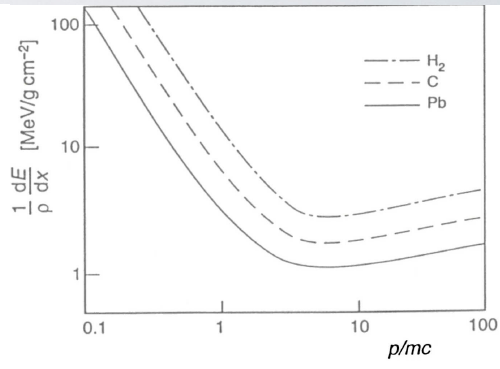
\includegraphics[scale=0.60]{Images1/perteenergie.PNG}
    \caption{Perte d'énergie par ionisation de quelques éléments}
    \label{fig:perte_energie}
\end{figure}

Un calcul plus précis, tenant compte des effets relativistes, et des corrections de densité de charge $\delta$ et $\dfrac{C}{Z}$, a été réalisé par Bethe et Block, et donne:
\[
    -\dfrac{1}{\rho}\fdif{E}{x} = K\dfrac{z^2}{\beta^2}\dfrac{Z}{A} \left[\ln\left(\dfrac{2m_ec^2\beta^2\gamma^2}{I}\right) - \beta^2-\dfrac{\delta}{2} -\dfrac{C}{Z}\right]
\]
où $K=\SI{0.307075}{MeV~g^{-1}~cm^2}$.

\begin{itemize}[label=$\longrightarrow$]
    \item \textbf{La correction de densité de charge} $\delta$ est due au fait que le champ électrique de la particule incidente polarise les atomes près de sa trajectoire. Cette polarisation réduit l'effet du champ électrique sur les électrons les plus éloignés (effet d'écran). Cela réduit la perte d'énergie. Cet effet est plus important si l'énergie des particules augmente (car le champ électrique est plus étendu), ou si la densité du matériau est plus élevée.
    \item \textbf{La correction $\dfrac{C}{Z}$} tient compte des effets de liaison des électrons et est importante à basse énergie.
\end{itemize}

\begin{rem}
    Cette formule met bien en évidence les dépendances de $\fdif{E}{x}$: le terme en $\dfrac{z^2}{\beta^2}$ montre la dépendance en la particule incidente (exemple: une particule $\alpha$ perd 4 fois plus d'énergie qu'un proton, pour un même $\beta$ et un même milieu), et celui en $\dfrac{Z}{A}$ montre la dépendance du milieu.
\end{rem}
\begin{rem}
    La relation entre $\fdif{E}{x}$ et la profondeur de pénétration est appelée courbe de Bragg. La dépendance en $1/v^2$ est marquée par la présence d'un pic appelé pic de Bragg (Figure \ref{fig:pic_bragg}). Cette caractéristique est utilisée en physique médicale dans le traitement de certaines tumeurs (on s'arrange pour que le pic de Bragg arrive pile à l'endroit de la tumeur et lui délivre donc toute son énergie).
\end{rem}

\begin{figure}[H]
    \centering
    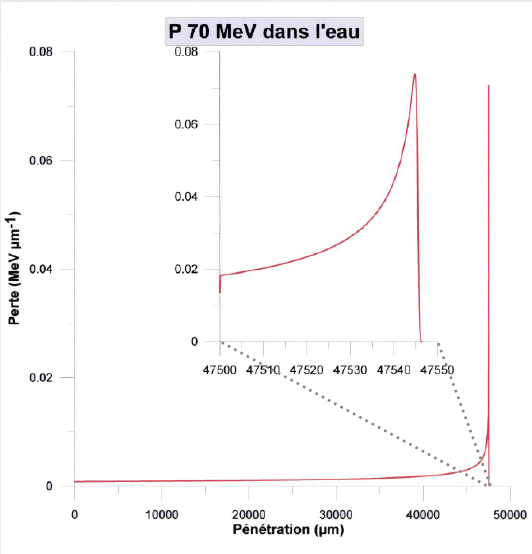
\includegraphics[width=0.5\textwidth]{Images1/picbragg.PNG}
    \caption{Courbe de Bragg théorique pour des protons de 70 \si{MeV} dans l'eau}
    \label{fig:pic_bragg}
\end{figure}

\begin{figure}[H]
    \centering
    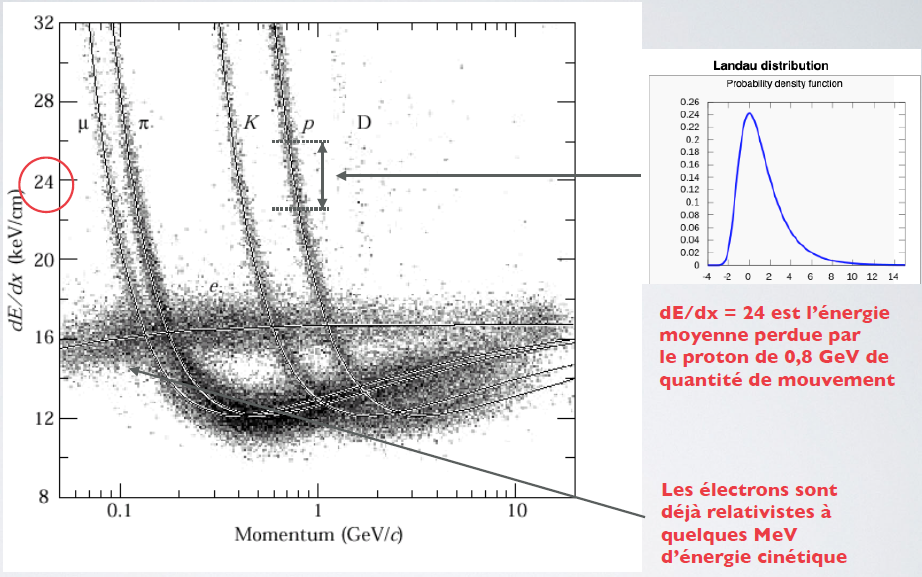
\includegraphics[width=0.66\textwidth]{Images1/perteionisation.PNG}
    \caption{Perte d'énergie par ionisation}
    \label{fig:pertes_ionisation}
\end{figure}

\subsubsection{Perte d'énergie par radiation}
À très haute énergie, les pertes d'énergie par collision deviennent négligeables par rapport aux pertes par radiation. Cet effet n'est important que pour les particules légères.

\begin{figure}[ht]
    \centering
    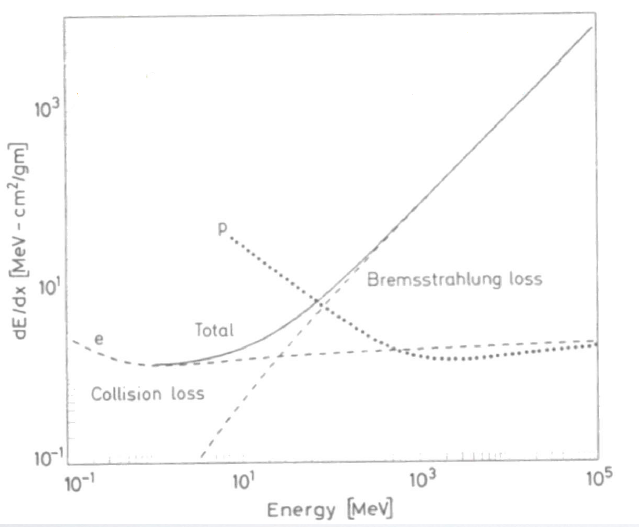
\includegraphics[scale=0.40]{Images1/bremstrucmachin.png}
    \caption{Pertes par collision et par radiation pour des électrons dans du cuivre}
    \label{fig:pertes_collision}
\end{figure}

La courbe qui monte linéairement (attention : graphe logarithmique) en pointillés est le Bremsstrahlung, le rayonnement de freinage qui correspond à l'interaction avec les noyaux n'ayant lieu qu'à hautes énergies, ce qui correspond également au domaine de valeur où la perte par ionisation ou collision (avec les e- des particules cibles) est négligeable. La courbe de cette interaction représentée en pointillés également et est plus ou moins plate, mais remonte à gauche, la zone où elle est prépondérante n'est en fait pas représenté sur le schéma. Le graphe montre également le comportement d'un proton qui réagit donc de manière opposée lors de ces interactions.\\
On constate que quand l'électron devient relativiste ($E>>m$), le rayonnement de freinage (Bremsstrahlung) domine rapidement. Les électrons perdent donc leur énergie par collision sur les électrons du milieu (Möller) et par diffusion élastique sur les noyaux (Mott): il y a déviation de leur trajectoire initiale et rayonnement de freinage. Le rayonnement de freinage varie en $Z^2$ de la cible.

\begin{figure}[ht]
    \centering
    \begin{subfigure}{.5\textwidth}
        \raggedright
        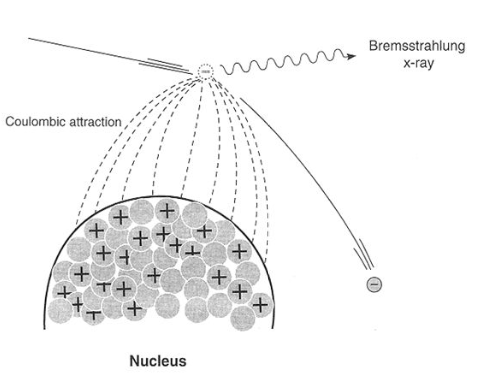
\includegraphics[width=.9\linewidth]{Images1/Bremsstrahlung2.PNG}
        %\caption{A subfigure}
        %\label{fig:sub1}
    \end{subfigure}%
    \begin{subfigure}{.5\textwidth}
        \raggedleft
        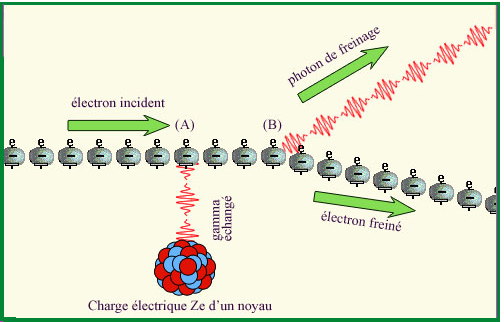
\includegraphics[width=.9\linewidth]{Images1/Bremsstrahlung3.PNG}
        %\caption{A subfigure}
        %\label{fig:sub2}
    \end{subfigure}
    \caption{Mécanisme du rayonnement de freinage}
    \label{fig:rayonnement_freinage}
\end{figure}

\paragraph{Notes supplémentaires sur le Bremsstrahlung:} Le phénomène de rayonnement de freinage (Fig. \ref{fig:rayonnement_freinage}) (Bremsstrahlung en allemand) concerne des particules porteuses d’une charge électrique dont la vitesse est proche de la vitesse de la lumière. Il intervient quand cette particule ultrarelativiste interagit avec un fort champ électrique ou magnétique, qui peut être naturel (le champ électrique d’un noyau) ou produit par l’homme (le champ d’aimants dans un accélérateur de particules). Les électrons et positons qui atteignent facilement des vitesses proches de celle de la lumière du fait de leur très faible masse sont les premiers concernés par le phénomène. \\

Le rayonnement de freinage intervient peu dans le domaine de la radioactivité, les électrons des désintégrations bêta n'étant souvent pas assez énergiques. Par contre, il joue un rôle important dans le rayonnement cosmique et le fonctionnement des accélérateurs de particules. \\

Sous l’effet de l’interaction, l’électron ou le positon, émets un photon qui emporte une partie de son énergie. L’électron est freiné et sa trajectoire modifiée. Le rayonnement de freinage est à l’origine d’une déperdition d’énergie dans de grands accélérateurs de particules comme les collisionneurs où les particules sont soumises à l’action de puissants aimants qui courbent leur trajectoire. Les ingénieurs des accélérateurs doivent compenser en permanence cette déperdition.

\subsubsection{Perte d'énergie des photons}
\begin{figure}[ht]
    \centering
    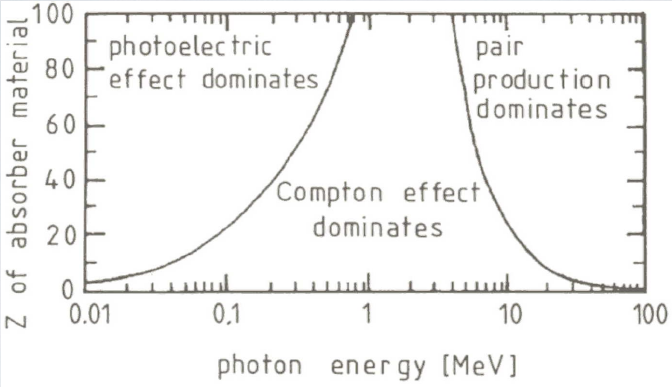
\includegraphics[scale=0.60]{Images1/pertephotons.PNG}
    \caption{Perte d'énergie des photons dans la matière}
    \label{fig:pertes_energie_photos}
\end{figure}
On constate bien sur la figure \ref{fig:pertes_energie_photos} que l'effet Compton est en compétition avec l'effet photoélectrique et la production de paires dans la perte d'énergie par les photons dans la matière\\

La diffusion Compton correspond à la collision d’un photon et d’un électron : le photon rebondit sur un électron cible qui est mis en mouvement et perd de l’énergie. L'électron est arraché à la matière, qui est donc ionisée, et le photon est diffusé. L'effet Compton contribue à l'atténuation des rayons gammas.  Arthur Compton a, en 1923, observé l'allongement de la longueur d'onde du photon dans cette diffusion, effet auquel on a attribué son nom : l'effet Compton.

\begin{figure}[ht]
    \centering
    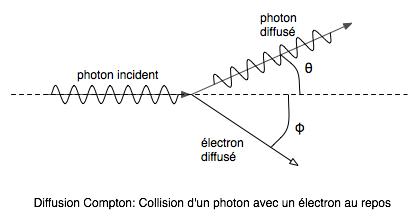
\includegraphics[scale=0.60]{Images1/compton.png}
    \caption{Diffusion Compton}
\end{figure}

La longueur d'onde change selon la formule
\[
    \lambda_f-\lambda_i=\dfrac{h}{m_ec}(1-\cos{\theta})
\]

\subsection{Découverte des rayonnements $\alpha$, $\beta$, $\gamma$}
\subsubsection{Radioactivité}
La radioactivité est le phénomène physique selon lequel des noyaux atomiques instables se transforment spontanément en d'autres atomes (désintégration) en émettant simultanément des particules de matière (électrons, noyaux d'hélium, neutrons, etc.) et de l'énergie (photons et énergie cinétique). Elle a été découverte en 1896 par Henri Becquerel dans le cas de l'uranium, et très vite confirmée par Marie Curie pour le radium. \\

Becquerel étudie le phénomène de phosphorescence. On connaissait déjà ce phénomène via lequel des matériaux émettent de la lumière dans le noir après avoir été exposés à la lumière (éventuellement des rayons X, découverts peu avant). Or, comme expliqué ci-dessus, Becquerel constata le noircissement des émulsions même en l'absence d'exposition à la lumière de sels d'uranium. Il y a donc des substances naturellement radioactives. Serait-ce donc une nouvelle émission similaire aux rayons X ? Quand on met ces substances naturellement radioactives dans une boîte blindée percée d'un petit trou, on observe 3 types de rayonnements: <<positif>>, <<neutre>>, et <<négatif>>, respectivement les rayonnements $\beta$, $\gamma$ et $\alpha$ (Fig. \ref{fig:alpha_beta_gamma}). Ils sont plus ou moins pénétrants dans la matière.

\begin{figure}[ht]
    \centering
    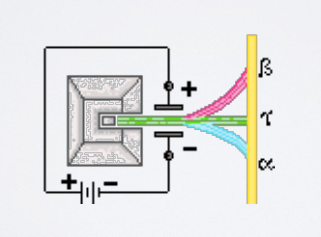
\includegraphics[width=0.4\textwidth]{Images1/rayonnements.PNG}
    \caption{Rayonnements $\alpha$, $\beta$, $\gamma$}
    \label{fig:alpha_beta_gamma}
\end{figure}

\begin{itemize}
    \item \textbf{Rayonnements $\alpha$}: Très vite arrêté par la matière (après une feuille de papier), spectre en énergie sous forme de raies dépendant de l'élément, produits par désintégration $\alpha$. C'est la forme de désintégration radioactive où un noyau atomique X éjecte une particule alpha (forme de rayonnement émis par des noyaux instables de grande masse atomique constitué de deux protons et deux neutrons combinés en une particule identique au noyau d'hélium 4 (hélion)) et se transforme en un noyau Y  de nombre de masse diminué de 4 et de numéro atomique diminué de 2. \\
    Forme générale:
    \[
        ^{A}_{Z}X \longrightarrow ^{A-4}_{Z-2}Y + ^{4}_{2} He ~ (+Q)
    \]
    Exemple:
    \[
        ^{238}U \longrightarrow ^{234}Th + \alpha
    \]
    Bilan énergétique d'une désintégration $\alpha$:
    \[
        Q = T_Y + T_\alpha = [M_{at}(X)-M_{at}(Y)-M_{at}(He)]c^2>0
    \]
    \[
        Q=B(A-4,Z-2)+B(^{4}_{2}He)-B(A,Z)>0
    \]

    \item \textbf{Rayonnements $\beta$}: La radioactivité bêta ou émission bêta est un type de désintégration radioactive dans laquelle une particule bêta (un électron ou un positon) est émise. Aujourd'hui, la désintégration $\beta$ se généralise à toutes les réactions nucléaires impliquant les neutrinos ou antineutrinos. Elle possède un plus grand pouvoir de pénétration (quelques millimètres), et est difficile à observer. Son spectre d'énergie est continu.

    Dans le cas du rayonnement $\beta$, si on trace le graphe de l'énergie des particules (Fig \ref{fig:spectre_beta}), on observe que la conservation de l'énergie n'est pas respectée. C'est ce constat qui inspira l'hypothèse de l'existence du neutrino.

    \begin{figure}[ht]
        \centering
        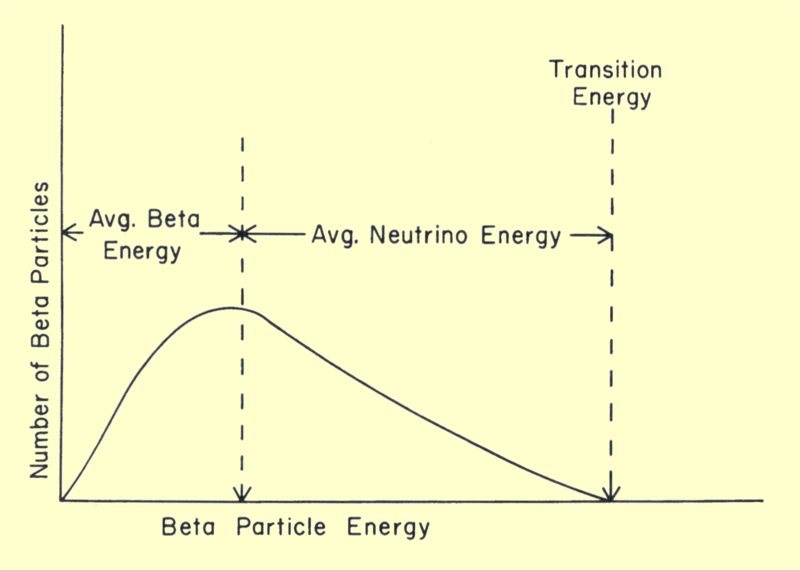
\includegraphics[scale=0.25]{Images1/beta.png}
        \caption{Spectre en énergie de la particule $\beta$}
        \label{fig:spectre_beta}
    \end{figure}

    On parle de désintégration bêta moins ($\beta^{-}$) ou bêta plus ($\beta^{+}$) selon qu'il s'agit de l'émission d'un électron ou d'un positon. Dès lors, on a respectivement les désintégrations suivantes :

    Forme générale:

    \[
        ^{A}_{Z}X \longrightarrow ^{A}_{Z+1}Y + e^- + \bar{\nu}_e
    \]

    \[
        ^{A}_{Z}X \longrightarrow ^{A}_{Z-1}Y + e^+ + \nu_e
    \]

    Exemple:
    \[
        ^{60}_{}Co \longrightarrow ^{60}_{}Ni^{+} + e^- + \bar{\nu}_e
    \]

    \[
        ^{18}_{}F \longrightarrow ^{18}_{}O + e^+ + \nu_e
    \]

    Il peut être intéressant de préciser que l'effet final d'un rayonnement Beta, pour un noyau radioactif instable, est de stabiliser le noyau (rétablir une balance n/p) en convertissant un neutron en proton et inversement (donc en émettant un e$^+$ ou e$^-$).

    \item \textbf{Rayonnements $\gamma$:} Possèdent un pouvoir de pénétration supérieur aux rayonnements alpha et beta et rayons X (ils passent quelques centimètres de plombs), spectre énergétique sous forme de raies. Le mécanisme de production des rayons $\gamma$ est illustré à la figure \ref{fig:rayons_gamma}.
\end{itemize}
\begin{figure}[ht]
    \centering
    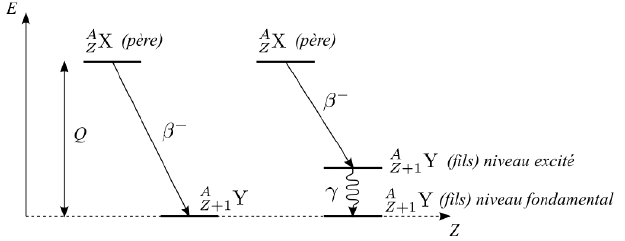
\includegraphics[width=0.8\textwidth]{Images1/gamma.PNG}
    \caption{Rayonnement $\gamma$}
    \label{fig:rayons_gamma}
\end{figure}
Les différents rayonnements obéissent à la loi de désintégration. Leur absorption est également exponentielle:
\[
    I(d)=I_0e^{-\mu d}
\]
où $\mu$ est un coefficient d'absorption\footnote{Ouais il a juste repris de Wikipédia. C'est quand ils passent dans la matière, ils sont absorbés de manière exponentielle et le mu dépend du matériau.}.


\section{Structure du noyau}
\subsection{Concept de section efficace}\label{sec:section_efficace}
\subsubsection{Définition}
Le concept de section efficace (Fig. \ref{fig:section_efficace}) couramment utilisé en physique nucléaire. C'est une grandeur physique reliée à la probabilité d'interaction d'une particule pour une réaction donnée. Son unité est le barn ($1b=10^{-24}cm^2$).
Quand on envoie un faisceau de particules, qu'on assimile à des sphères dures sur une cible, la probabilité d'interaction avec celle-ci est
\[
    \delta P_{int}=\dfrac{\text{Surface des sphères projetées}}{\text{Surface totale}}=\delta N \dfrac{\pi r^2}{S}=n \dif x \pi r^2
\]
où
\begin{itemize}
    \item $\delta N$ est le nombre de boules vues pour une surface S
    \item n est la densité volumique de sphères
    \item $\dif x$ est l'épaisseur de la cible
    \item $\sigma=\pi r^2$ est la section efficace géométrique
\end{itemize}

\begin{figure}[ht]
    \centering
    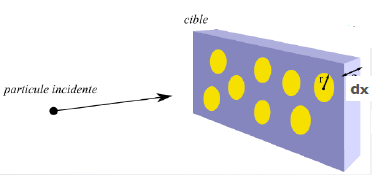
\includegraphics[scale=0.75]{Images1/section_efficace.PNG}
    \caption{Concept de section efficace}
    \label{fig:section_efficace}
\end{figure}
Si on a $N_i$ particules incidentes et $\dif N$ interactions pour une cible d'épaisseur $\dif x$, on admet comme définition de $\sigma$
\[
    \dif N=-N_in\sigma \dif x
\]
La section efficace ne dépend que du projectile et de la cible élémentaire. Pour une section efficace géométrique de l'ordre de \SI{100}{mb}, on a $r_o=\sqrt{\dfrac{\sigma}{\pi}}\sim \SI{e-15}{m} = \SI{1}{fm}$, ce qui est la taille typique des nucléons. Cela explique que, $\sigma(p+\text{noyau})\propto A^{2/3}$ car rayon du noyau $\propto A^{1/3}$.

\subsubsection{Section efficace d'interaction et temps de vie}
On considère une cible de surface S sur laquelle sont projetées des particules pendant une expérience. La section efficace pour cette réaction est $\sigma$. Si $n_0$ est le nombre de noyaux cibles par \si{cm^3}, alors le nombre total de noyaux cibles est $n_0 V$ = $n_0 S x$ et la section efficace de toutes les cibles est $\sigma_{tot}$ = $\sigma n_0 S X$. On peut donc déduire la probabilité qu'il y ait une réaction:
\[
    P=\dfrac{\sigma_{tot}}{S}
\]
et, sachant que $I$ est le nombre de particules incidentes durant toute l'expérience, le nombre de réactions durant l'expérience
\[
    N=I \sigma n_0 x
\]
Définissons maintenant la section efficace en tenant compte des composantes angulaires lors de la diffusion de la particule (Fig. \ref{fig:diffusion_particule}).

\begin{figure}[ht]
    \centering
    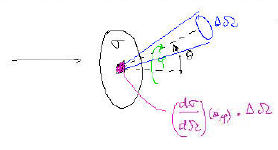
\includegraphics[scale=0.95]{Images1/secdiff.PNG}
    \caption{Représentation de la diffusion d'une particule}
    \label{fig:diffusion_particule}
\end{figure}
\noindent La section efficace telle que la particule part dans l'angle solide $\Delta\Omega$ centré sur $\theta$, $\phi$ est
\[
    \sigma=\int_{4\pi}^{}\fdif{\sigma}{\Omega}\dif \Omega
\]
où $\fdif{\sigma}{\Omega}$ est la section efficace différentielle. On a donc pour le nombre de réactions durant l'expérience
\[
    \dif N=I~n_0~X~\Big(\fdif{\sigma}{\Omega}\Big)~\Delta\Omega \quad\text{avec}\quad \fdif{\sigma}{\Omega}=\dfrac{\dif\sigma}{\dif\phi \dif \;(\cos{\theta})}=\dfrac{1}{2\pi}\fdif{\sigma}{\;(\cos{\theta})}
\]
Pour se représenter la situation, le détecteur correspond à un anneau réalisant toute une révolution autour de l'axe de l'expérience avec un avec $\phi$ (la direction de propagation des particules incidentes) et cela à un certain angle $\theta$.

\subsubsection{Longueur d'atténuation}
On a $\dif N=I_0 n_0 \sigma \dif x=-\dif I$. Si on intègre, on obtient
\[
    \int_{I_{0}}^{I(x)}\dfrac{\dif I}{I}=-\int_0^x n_0.\sigma \dif x
\]
c'est-à-dire que
\[
    I(x)=I_0e^{-n_0.\sigma.x}=I_0.e^{-x/x_0}
\]
On définit $x_0=\dfrac{1}{n_0\sigma}$ comme la longueur d'atténuation.

\subsubsection{Section efficace différentielle}
La section efficace (et donc la probabilité d'interaction) dépend de paramètres géométriques tels que le flux de particules uniforme dans le plan perpendiculaire à la direction de propagation $\Phi=\dfrac{\dif^2N}{\dif t\dif s}$, le nombre de particules diffusées par unité de temps et par unité d'angle solide dans la direction $(\theta, \theta+\dif \theta)$.
\begin{figure}[ht]
    \centering
    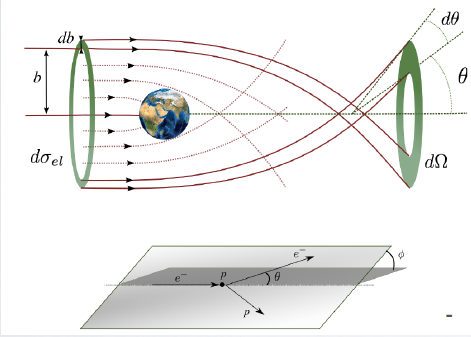
\includegraphics[scale=0.75]{Images1/section_efficace_diff.PNG}
    \caption{Concept de section efficace différentielle}
    \label{fig:section_efficace_diff}
\end{figure}
On a
\[
    \dfrac{\dif^2N}{\dif t\dif \Omega}=\dfrac{\dif^2N}{\dif t\dif \sigma_{el}} \fdif{\sigma_{el}}{\Omega}
\]
Si on mesure le nombre d'électrons à $\theta$ fixé,
\[
    \fdif{\sigma_{el}}{\Omega}=\dfrac{2\pi~b~\dif b}{2\pi \sin{\theta}\dif \theta}
\]
et à angle solide fixé,
\[
    \dif N=N_i~n~\dif x~\dif \Omega~\fdif{\sigma}{\Omega}
\]

\begin{figure}[ht]
    \centering
    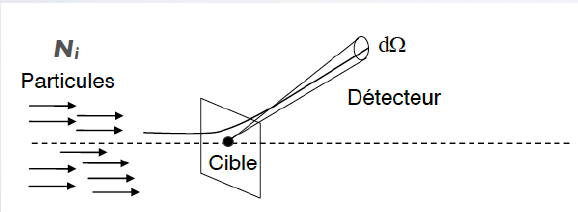
\includegraphics[scale=0.75]{Images1/anglesolide.PNG}
    \caption{Angle solide fixé}
\end{figure}
Remarquons que
\[
    \int(\fdif{\sigma}{\Omega})\dif \Omega=\sigma_{tot}
\]
Du fait de la symétrie, toutes les particules qui ont des paramètres d'impact compris entre $b$ et $b+\dif b$ seront diffusées entre $\theta$ et $\theta+\dif\theta$. Elles sont donc associées à une <<surface>> $2\pi b\cdot \dif b$ perpendiculaire au faisceau (figure \ref{fig:surface_de_diffusion}).
\begin{figure}[ht]
    \centering
    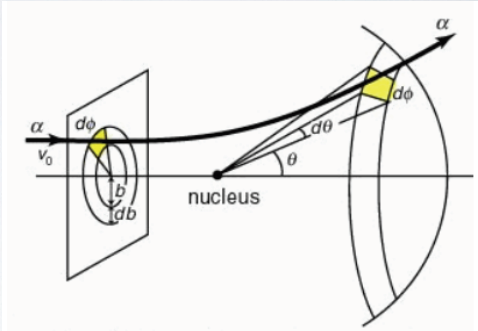
\includegraphics[scale=0.75]{Images1/surface_perp.PNG}
    \caption{<<Surface de diffusion>>}
    \label{fig:surface_de_diffusion}
\end{figure}
Pour une épaisseur x
\[
    \dif N=N_i~n_{\text{cible}}~x~\left(\fdif{\sigma}{\Omega}\right)\dif \Omega
\]
Si on intègre sur l'angle phi, on obtient la définition de \textbf{section efficace différentielle}
\[
    \fdif{\sigma}{\Omega}=\dfrac{2\pi b \dif b}{\dif \Omega}=\dfrac{2\pi~b~\dif b}{2\pi \sin{\theta}\dif\theta}=\dfrac{b}{\sin{\theta}}\abs{\fdif{b}{\theta}}
\]

\subsubsection{Section efficace de Rutherford}
Le développement est très bien expliqué sur \url{http://res-nlp.univ-lemans.fr/NLP_C_M13_G01/co/Contenu17.html}. L'auteur ne fait pas tout à fait comme Lemaître, mais arrive au même résultat.

\subsubsection{Expérience de Geiger et Marsden}
Cette expérience montra que la partie chargée positivement de la matière est concentrée en un espace de petit volume, le noyau atomique. L'expérience est réalisée sous vide. De la matière radioactive émettant des particules $\alpha$ est placée dans une boîte et le faisceau de particules $\alpha$ est orienté en direction d'une très fine feuille d'or (6 000 $\angstrom$). Derrière cette couche d'or, un écran est placé ; il est enrichi d'une substance chimique permettant de visualiser, par un scintillement lumineux, la collision par les particules $\alpha$ (Fig. \ref{fig:geiger_marsden}).

\begin{figure}[ht]
    \centering
    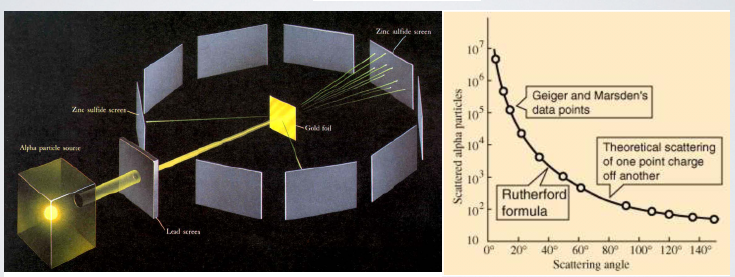
\includegraphics[scale=0.75]{Images1/geiger.PNG}
    \caption{Expérience de Geiger et Marsden : Dispositif - Comparaison prédictions/mesures}
    \label{fig:geiger_marsden}
\end{figure}

Plusieurs minutes après la disposition du matériel, différents points lumineux apparaissent sur l'écran et ces points ne sont pas tous dans l'orientation du faisceau, mais certains étalés sur de grands angles. Rutherford eut ainsi la surprise d'observer une sorte de rebond des particules alpha.

La rétrodiffusion de particules $\alpha$ ne peut s’expliquer que par des chocs élastiques entre les particules alpha et des noyaux atomiques beaucoup plus massifs! Le modèle atomique du flan aux raisins ne résiste évidemment pas à ces observations qui mèneront au modèle de Rutherford (Fig. \ref{fig:mod_rutherford}).
\begin{figure}[ht]
    \centering
    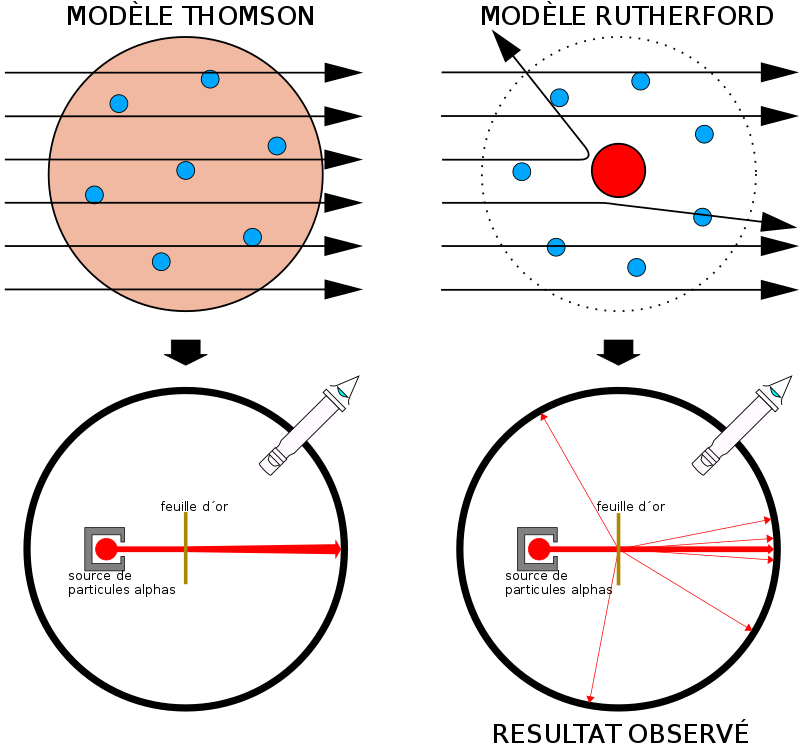
\includegraphics[scale=0.25]{Images1/thom_ruth.png}
    \caption{Modèle de Thomson VS modèle de Rutherford}
    \label{fig:mod_rutherford}
\end{figure}
La distance d'approche minimale calculée par Rutherford satisfait à l'équation

$$\dfrac{1}{2}mv_0^2=\dfrac{1}{4\pi\epsilon_0}\dfrac{Zze^2}{r_\text{min}}$$

Si on projette des $\alpha$ de plus haute énergie sur du plomb par exemple, on observe une diminution du nombre de particules rétrodiffusées à cause de l'interaction forte à courte distance. En effet, les $\alpha$ sont alors absorbés par les noyaux.

\subsection{Découverte du proton}
En 1914, on veut élaborer une théorie du noyau. De quels éléments dispose-t-on ? Le numéro atomique Z, la masse atomique A, le fait qu'un même élément chimique puisse exister sous forme de plusieurs isotopes avec A différents, la radioactivité alpha (il y a des particules alpha, qui sont des noyaux d'hélium, dans certains noyaux), la radioactivité beta (il y a des particules beta, qui sont des électrons, dans certains noyaux). \\
En 1911, Rutherford part des 2 observations que pour la plupart des noyaux, $A \sim 2Z$ et que certains noyaux émettent des particules alpha. Il suggère donc que tous les noyaux, hormis l'hydrogène, sont des assemblages de particules alpha. \\
Cependant, beaucoup d'arguments s'opposent à cette théorie: la moitié des charges électriques Z sont impaires, les masses de la plupart des éléments lourds sont supérieures au double de leur charge électrique, et l'écart s'accroit avec la masse (exemple: du Fer A=56, Z=26 au Plomb A=207, Z=82).  Cela suggère un modèle mixte: hélium + autre chose ? Alors, pourquoi ne pas former directement les noyaux par des assemblages de noyaux d'hydrogène, puisque la plupart des masses atomiques sont des multiples entiers de la masse de l'hydrogène ? Il existe une objection majeure à cette proposition : si on forme le noyau de masse A avec A noyaux d'hydrogène, ce noyau a une charge électrique +Ae, et non +Ze... Rutherford suppose alors à l'époque que le noyau possède en plus A-Z électrons, ce qui expliquerait en plus que les noyaux perdent des électrons dans la radioactivité beta. Cette théorie du noyau avait 2 conséquences:

\begin{itemize}
    \item Il y a des noyaux d'hydrogène dans TOUS les noyaux
    \item Il doit exister un mécanisme séparant les Z électrons dits périphériques des A-Z électrons nucléaires.
\end{itemize}

Le premier point a des conséquences expérimentales un peu étranges que Rutherford mit en avant: en 1915, avec Marsden il bombarde de l'hydrogène avec des particules alpha (source = radon), à l'aide du dispositif illustré ci-dessous. La chambre est remplie de gaz, une source d’alphas (la plaque sur le pied) les projette sur les noyaux du gaz (Fig. \ref{fig:chambre_bombardement_H}). Les alphas, les noyaux du gaz et les protons provoquent des scintillations différentes sur l’écran de sulfure de zinc à droite, observé au microscope. Ils observent des reculs de l'hydrogène, caractérisés par des traces plus fines que celles des alphas.

\begin{figure}[ht]
    \centering
    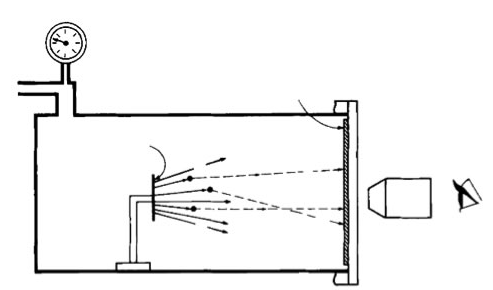
\includegraphics[scale=0.75]{Images1/bombardement.PNG}
    \caption{Chambre de bombardement d'hydrogène}
    \label{fig:chambre_bombardement_H}
\end{figure}

Marsden remarqua une émission d'hydrogène par le radon avant le remplissage de la chambre en hydrogène. Rutherford ne crut pas à une nouvelle forme de radioactivité, mais plutôt à une contamination de l'appareillage par l'hydrogène. Il nota plus tard que s'il remplissait la chambre d'oxygène ou de gaz carbonique, le nombre de scintillations attribuables à l'hydrogène diminuait, comme il s'y attendait, mais ce nombre augmentait quand la chambre était remplie d'air et plus encore quand elle était remplie d'azote ! Ce phénomène de <<fuite d'hydrogène>> n'apparaissait que pour des alphas d'énergie supérieure à 1.21 \si{MeV}. Rutherford supposa donc une ionisation des molécules d'eau présentes dans l'air ou l'azote. Mais après suppression de l'eau, le phénomène persistait, Rutherford en conclut donc que l'azote se transmutait au cours de la collision avec les alphas, et que les noyaux d'hydrogène appartenaient au noyau d'azote. Rutherford pensait observer la réaction
\begin{center}
    alpha + azote $\longrightarrow$ hydrogène + carbone + alpha
\end{center}
et son interprétation fut la suivante en 1919 :

\begin{itemize}
    \item Carbone: masse atomique 12 = 3 alphas
    \item Oxygène: masse atomique 16 = 4 alphas
    \item Azote: masse atomique 14 = 3 alphas + 2 hydrogènes périphériques, facilement arrachables par l’alpha servant de projectile, dès qu’il avait une énergie suffisante (les 1.21 \si{MeV} requis)
\end{itemize}

Cette interprétation a 2 conséquences majeures: les transmutations nucléaires ne sont pas limitées aux éléments lourds (radioactifs) et les collisions d'alphas permettent de sonder en profondeur les noyaux, pas seulement leur cortège d'électrons.

Rutherford a ainsi développé une nouvelle technique de recherche, malheureusement limitée par la faible énergie des alphas. S'en suivit pour remédier à ce problème la conception d'accélérateurs, comme le premier cyclotron, par Lawrence (Fig. \ref{fig:lawrence_cyclo}).

L’utilisation de la chambre de Wilson (ou chambre à brouillard) (Fig. \ref{fig:chambre_wilson}) se révéla bien plus pratique que les écrans au sulfure de zinc, car elle permettait de visualiser, et d’enregistrer, le résultat des collisions sous la forme de traces des particules avant et après collision, et même parfois de mesurer leur charge et leur énergie. En 1920, Chadwick mesura la charge des noyaux Cu, Ag, Pt par diffusion alphas. Ayant démontré qu’il y avait bien des noyaux d’hydrogène dans le noyau d’azote, Rutherford les baptisa proton en 1920.

\begin{figure}[ht]
    \centering
    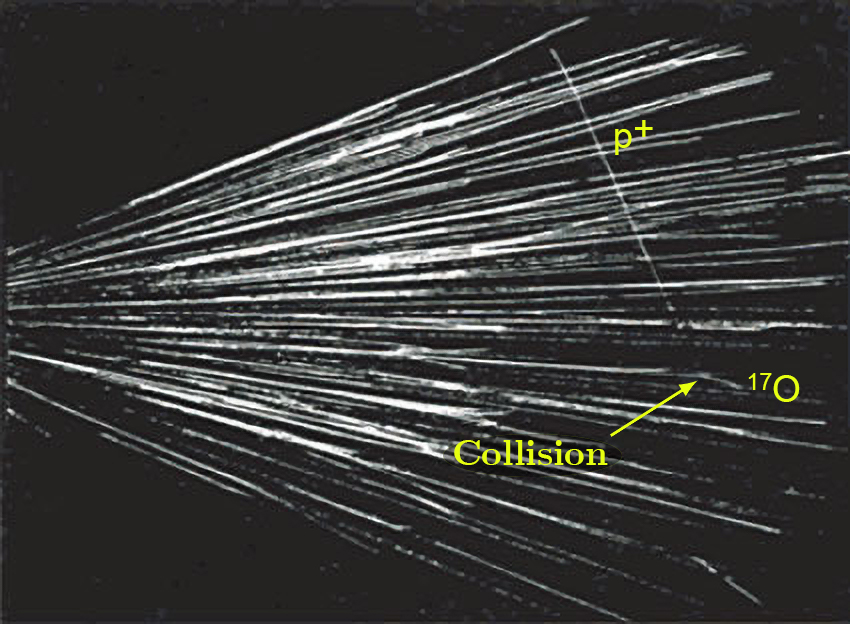
\includegraphics[width=0.7\textwidth]{Images1/collisions_alpha_proton.jpg}
    \caption{La chambre à brouillard de Wilson: des particules alpha provenant d'une source sur la gauche laissent une traînée des gouttelettes dans une chambre à brouillard remplie d'azote. L'une d'entre elles frappe un noyau d'azote à droite, donnant un proton partant vers le haut gauche et un noyau d'oxygène partant vers le bas à droite. (Blackett 1935)}
    \label{fig:chambre_wilson}
\end{figure}

Les expériences de Rutherford validaient --- apparemment --- l’image du noyau comme un assemblage de A protons avec A-Z électrons <<nucléaires>>, associés pensait-il en sous-structures alpha. De nombreux modèles qualitatifs furent élaborés pour rendre compte des régularités empiriques, mais ils étaient peu prédictifs, et surtout ils entrèrent très vite en conflit avec la nouvelle mécanique quantique (Fig. \ref{fig:to_be_continued})...

\begin{figure}[ht]
    \centering
    \begin{minipage}{.5\textwidth}
        \centering
        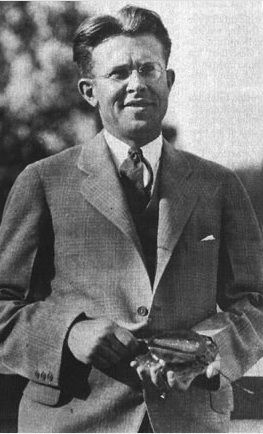
\includegraphics[height=5.5cm]{Images1/cyclo.PNG}
        \captionof{figure}{Lawrence et un bébé cyclotron}
        \label{fig:lawrence_cyclo}
    \end{minipage}%
    \begin{minipage}{.5\textwidth}
        \centering
        
\includegraphics[height=5.5cm]{Images1/mama.png}
        \captionof{figure}{To be continued...}
        \label{fig:to_be_continued}
    \end{minipage}
\end{figure}

\subsection{Découverte du neutron}
En gros:
\begin{itemize}
    \item 1931: Joliot et sa femme Curie bombardent du Béryllium avec une source d'alpha et observent une radiation très pénétrante (Fig. \ref{fig:joliot_curie}).

    \begin{figure}[H]
        \centering
        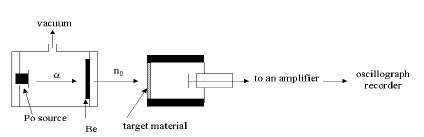
\includegraphics[scale=0.99]{Images1/joliotcurie.PNG}
        \caption{Expérience de Joliot-Curie}
        \label{fig:joliot_curie}
    \end{figure}

    Hypothèse de Bothe et Becker: ce sont des rayons X. Hypothèse de Joliot et Curie: ce sont des rayons gamma, et la réaction est donc similaire à celle de l'effet Compton sur des protons. Ils pensent cela, car ils observent l'émission de protons éjectés d'une cible de paraffine bombardée avec cette radiation. (protons mesurés avec une chambre à ionisation.) Hypothèse de Chadwick: la radiation correspond à une interaction avec une nouvelle particule neutre donc la masse est similaire à celle du proton selon la réaction
    \[
        ^{4}_{2}He + ^{9}_{4}Be \rightarrow ^{12}_{6}C + ^{1}_{0}n
    \]

    \item Il mesure que les protons éjectés ont des vitesses maximales $v=\dfrac{c}{10}$ dans une chambre à brouillard, compatible avec des photons de \SI{50}{MeV} incidents, ce qui est très élevé pour des rayons gamma qui ont normalement une énergie de quelques \si{MeV}.

    \item Il note le recul de noyaux d'azote si l'azote est introduit dans la chambre à brouillard (Fig \ref{fig:recul_azote}) ! Ici aussi, le parcours de l'azote dans le chambre est tel que l'énergie est bien plus élevée que 400 \si{keV} (qui serait l'énergie maximale si on avait des photons de \SI{50}{MeV})


    \begin{figure}[ht]
        \centering
        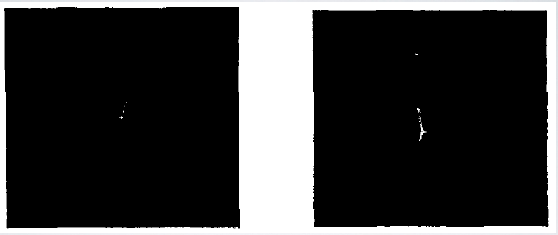
\includegraphics[scale=0.85]{Images1/reculazote.PNG}
        \caption{Gauche: Recul de ce qui pourrait être un ion d'azote - Droite: Recul d'un ion d'azote qui fait interaction élastique avec un autre noyau d'azote}
        \label{fig:recul_azote}
    \end{figure}

    \item Il observe aussi d'autres réactions inélastiques type $n + ^{14}N \rightarrow ^{11}B + \alpha $ (voir figure \ref{fig:coll_inelastique})

    \begin{figure}[ht]
        \centering
        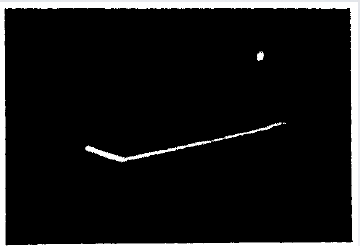
\includegraphics[scale=0.80]{Images1/inelastique.PNG}
        \caption{Réactions inélastiques entre un neutron et l'azote de la chambre}
        \label{fig:coll_inelastique}
    \end{figure}
\end{itemize}
Comment a-t-on déterminé la masse de la nouvelle particule, le neutron ? Pour la collision
\[
    m + M \rightarrow m + M
\]
où m a une vitesse initiale v et M est au repos, on a que la vitesse maximale de M après la collision est
\[
    \dfrac{2mv}{(m+M)}
\]
Sachant que les vitesses maximales pour le proton de recul et l'azote sont respectivement \SI{3.7e9}{cm/s} et \SI{1.7e8}{cm/s}, on obtient $m$ = $90\%~M_\text{proton}$. En bons physiciens, on considère donc que $M_\text{proton}$ = $M_{neutron}$. (En vrai, des mesures plus précises ont indiqué que la différence entre le deux vaut 0,14 pour cent de la masse moyenne du proton et du neutron.)

\subsection{Mesure de la masse des noyaux et énergie de liaison}
Expérimentalement, on détermine la masse des noyaux via la technique de spectrographie de masse (Fig. \ref{fig:spectro_masse}). Elle consiste à identifier les masses des composants d'un échantillon de manière individuelle grâce à un faisceau d'ions. Une source produit ce faisceau possédant une certaine distribution de vitesses. Un sélecteur de vitesses permet seulement aux ions ayant une vitesse particulière de passer (le reste du faisceau est défléchi), et la sélection de moments grâce à un champ magnétique permet l'identification des masses individuelles.
\begin{figure}[ht]
    \centering
    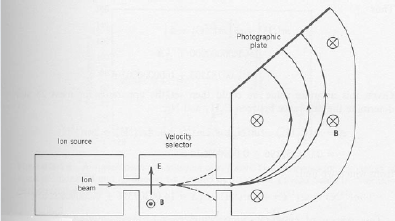
\includegraphics[scale=0.80]{Images1/spectro.PNG}
    \caption{Principe du spectrographe de masse}
    \label{fig:spectro_masse}
\end{figure}
Soit un atome avec A nucléons, Z protons et Z électrons. Sa masse M(A,Z) s'écrit
\[
    M(A,Z) = m(A,Z) + Z \cdot m_e - E^{\text{atome}}_{\text{liaison}}
\]
avec m(A,Z) la masse du noyau de l'atome, définie par
\[
m(A,Z)=Z.m_p+(A-Z)m_n-E^{\text{nucléaire}}_{\text{liaison}}
\]
Définissons l'énergie de liaison de l'atome par
\[
    B=E^\text{atome}_\text{liaison}+E^{\text{noyau}}_{\text{liaison}}
\]
Elle est largement dominée par l'énergie de liaison nucléaire de sorte que dans la suite, on approximera B comme l'énergie de liaison du noyau. Cette énergie de liaison est généralement négligeable devant l'énergie de masse.
En guise d'exemple, on considère le système de 2 nucléons (le deutérium). Évaluons l'énergie de liaison de son noyau, le deuton. On a
\[
    M(^{2}_{}D)=2.014~u
\]
où \[u=\dfrac{1}{12}M(^{12}_{}C)=931.495 \cdot \dfrac{\si{MeV}}{c^2}=\SI{1.66054e-27}{kg}\]
Connaissant les masses du proton, neutron et électron, on trouve que
\[
    B(^{2}_{}D) = \SI{2.227}{MeV}/c^2
\]
soit $0.12\%~M(^{2}_{}D)$.

\subsection{Découverte des rayons cosmiques et de l'antimatière}
Le rayonnement cosmique est le flux de noyaux atomiques et de particules de haute énergie (relativistes) qui circulent dans le milieu interstellaire. La source de ce rayonnement se situe selon les cas dans le Soleil, à l'intérieur ou à l'extérieur de notre galaxie. Certaines astroparticules qui composent le rayonnement cosmique ont une énergie qui dépasse 1020 eV et qui n'est expliquée par aucun processus physique identifié. Le rayonnement cosmique est principalement constitué de particules chargées : protons, noyaux d'hélium, antiprotons, électrons, positrons et particules neutres (rayons gamma, neutrinos et neutrons).\\[0,2cm]
La découverte du rayonnement cosmique a lieu au début du XXe siècle avec les observations de Victor Hess effectuées en 1912 depuis un ballon. Il observe une légère diminution du taux de décharge de l'électroscope entre 0 et 500m d'altitude (mesure effectuée initialement entre la base de la tour Eiffel et son sommet, à 324m d'altitude).

\begin{figure}[ht]
    \centering
    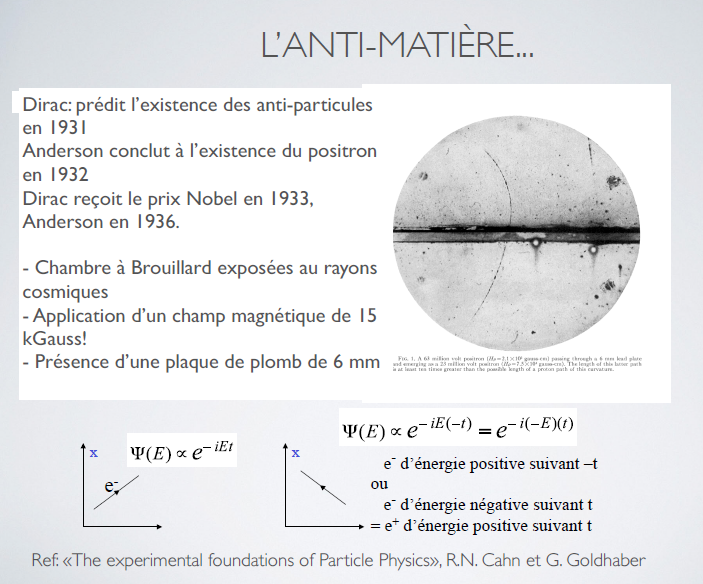
\includegraphics[scale=0.80]{Images1/antimatiere.PNG}
    \caption{Découverte de l'antimatière}
\end{figure}
\newpage
